\documentclass{report}

% Language setting
% Replace `english' with e.g. `spanish' to change the document language
\usepackage[utf8]{inputenc}
\usepackage[polish]{babel}
\usepackage[T1]{fontenc}

\usepackage{array}
\usepackage{booktabs}

% Set page size and margins
% Replace `letterpaper' with `a4paper' for UK/EU standard size
\usepackage[letterpaper,top=2cm,bottom=2cm,left=3cm,right=3cm,marginparwidth=1.75cm]{geometry}

% Useful packages
\usepackage{amsmath}
\usepackage{graphicx}
\usepackage[colorlinks=true, allcolors=black]{hyperref}

\usepackage{float}


\usepackage{listings}
\lstset{
  inputencoding=utf8,
  extendedchars=true,
  literate=
    {ą}{{\k{a}}}1
    {ć}{{\'c}}1
    {ę}{{\k{e}}}1
    {ł}{{\l{}}}1
    {ń}{{\'n}}1
    {ó}{{\'o}}1
    {ś}{{\'s}}1
    {ź}{{\'z}}1
    {ż}{{\.z}}1
    {Ą}{{\k{A}}}1
    {Ć}{{\'C}}1
    {Ę}{{\k{E}}}1
    {Ł}{{\L{}}}1
    {Ń}{{\'N}}1
    {Ó}{{\'O}}1
    {Ś}{{\'S}}1
    {Ź}{{\'Z}}1
    {Ż}{{\.Z}}1,
}

\usepackage{xcolor}

\definecolor{codegreen}{rgb}{0,0.6,0}
\definecolor{codegray}{rgb}{0.5,0.5,0.5}
\definecolor{codepurple}{rgb}{0.58,0,0.82}
\definecolor{backcolour}{rgb}{0.95,0.95,0.92}

\lstdefinestyle{mystyle}{
    backgroundcolor=\color{backcolour},   
    commentstyle=\color{codegreen},
    keywordstyle=\color{magenta},
    numberstyle=\tiny\color{codegray},
    stringstyle=\color{codepurple},
    basicstyle=\ttfamily\footnotesize,
    breakatwhitespace=false,         
    breaklines=true,                 
    captionpos=b,                    
    keepspaces=true,                 
    numbers=left,                    
    numbersep=5pt,                  
    showspaces=false,                
    showstringspaces=false,
    showtabs=false,                  
    tabsize=2
}

\lstset{style=mystyle}

\usepackage{tikz}
\usetikzlibrary{trees}
\usepackage{forest}
\usetikzlibrary{arrows.meta, shapes.geometric, positioning}

\usepackage{authblk}

\usepackage{enumitem}
\usepackage{float}
\usepackage{subcaption}

\title{\LARGE{Analiza skupień danych dotyczących cen mieszkań}
\vspace{0.3cm}
\Large{Metody Analizy Danych - zadanie projektowe 1}}

\author{
Joanna Dagil (231008),
Liliana Grześkiewicz (236138),
Piotr Szpatusko (223420),
Adam Włodarski (230983)
}

\date{rok akademicki 2025/2026}

\begin{document}

\maketitle

\tableofcontents

\chapter*{Streszczenie}
\addcontentsline{toc}{chapter}{Streszczenie}

Projekt polega na analizie zbioru danych z Kaggle zawierającego oferty sprzedaży i najmu mieszkań z 15 największych miast w Polsce.
Celem pracy jest wykorzystanie metody cluster do automatycznego wyodrębnienia grup podobnych ofert, ponieważ clustering należy do metod uczenia nienadzorowanego i służy do odkrywania ukrytych wzorców w danych bez gotowych etykiet.
Dzięki temu można wskazać segmenty rynku mieszkaniowego różniące się poziomem cen oraz podobieństwem ofert między miastami.
Taki projekt pomaga lepiej zrozumieć strukturę polskiego rynku mieszkań i stanowi dobrą podstawę do dalszej analizy trendów cenowych oraz porównań regionalnych.

\vspace{0.5cm}
\noindent\textbf{Słowa kluczowe:} analiza skupień, klastry, ceny mieszkań

\chapter{Wstęp}

Rynek nieruchomości w Polsce charakteryzuje się dużą dynamiką oraz znacznym zróżnicowaniem regionalnym. W obliczu stale rosnącej liczby ogłoszeń, tradycyjne metody przeglądania ofert stają się niewystarczające do pełnego zrozumienia mechanizmów rządzących tym sektorem. Niniejszy projekt podejmuje próbę uporządkowania i segmentacji tych danych przy użyciu zaawansowanych metod statystycznych.

Podstawę analizy stanowi zbiór danych pozyskany z serwisu Kaggle, obejmujący oferty sprzedaży oraz najmu mieszkań z 15 największych miast w Polsce. Ze względu na wielowymiarowość cech opisujących każdą nieruchomość, w pracy zdecydowano się na wykorzystanie metod uczenia nienadzorowanego.

\textbf{Głównym celem projektu} jest wykorzystanie metody analizy skupień do automatycznego wyodrębnienia grup podobnych ofert. Metoda ta pozwala na odkrywanie ukrytych wzorców w danych bez konieczności posiadania gotowych etykiet. Takie podejście umożliwia obiektywne wskazanie segmentów rynku mieszkaniowego, które różnią się poziomem cen oraz specyficznym podobieństwem cech fizycznych lokali.

W toku prac badanie zostało zawężone do rynku krakowskiego. Wybór Krakowa podyktowany jest faktem, że miasto to charakteryzuje się największą ilością ofert spośród wszystkich dostępnych miast, z wyłączeniem Warszawy. Większa ilość danych dostępnych dla tego regionu pozwala na uzyskanie bardziej reprezentatywnych wyników analizy skupień oraz lepsze zidentyfikowanie wzorców i grup w danych dotyczących cen mieszkań.

Realizacja projektu ma na celu:
\begin{itemize}
    \item lepsze zrozumienie struktury polskiego rynku mieszkań;
    \item identyfikację kluczowych segmentów rynku różniących się poziomem cen;
    \item stworzenie solidnej podstawy do dalszej analizy trendów cenowych oraz porównań regionalnych.
\end{itemize}

\chapter{Przedmiot badania}

Badanie ograniczymy do jednego z miast z dostepnych danych. Analizując ilość wynajmów w poszczególnych miastach, wybieramy miasto z największą ilością wynajmów (oprócz Warszawy), co pozwoli nam na uzyskanie bardziej reprezentatywnych wyników analizy skupień. Na poniższym wykresie przedstawiono ilość wynajmów w poszczególnych miastach.

\begin{figure}[H]
    \centering
    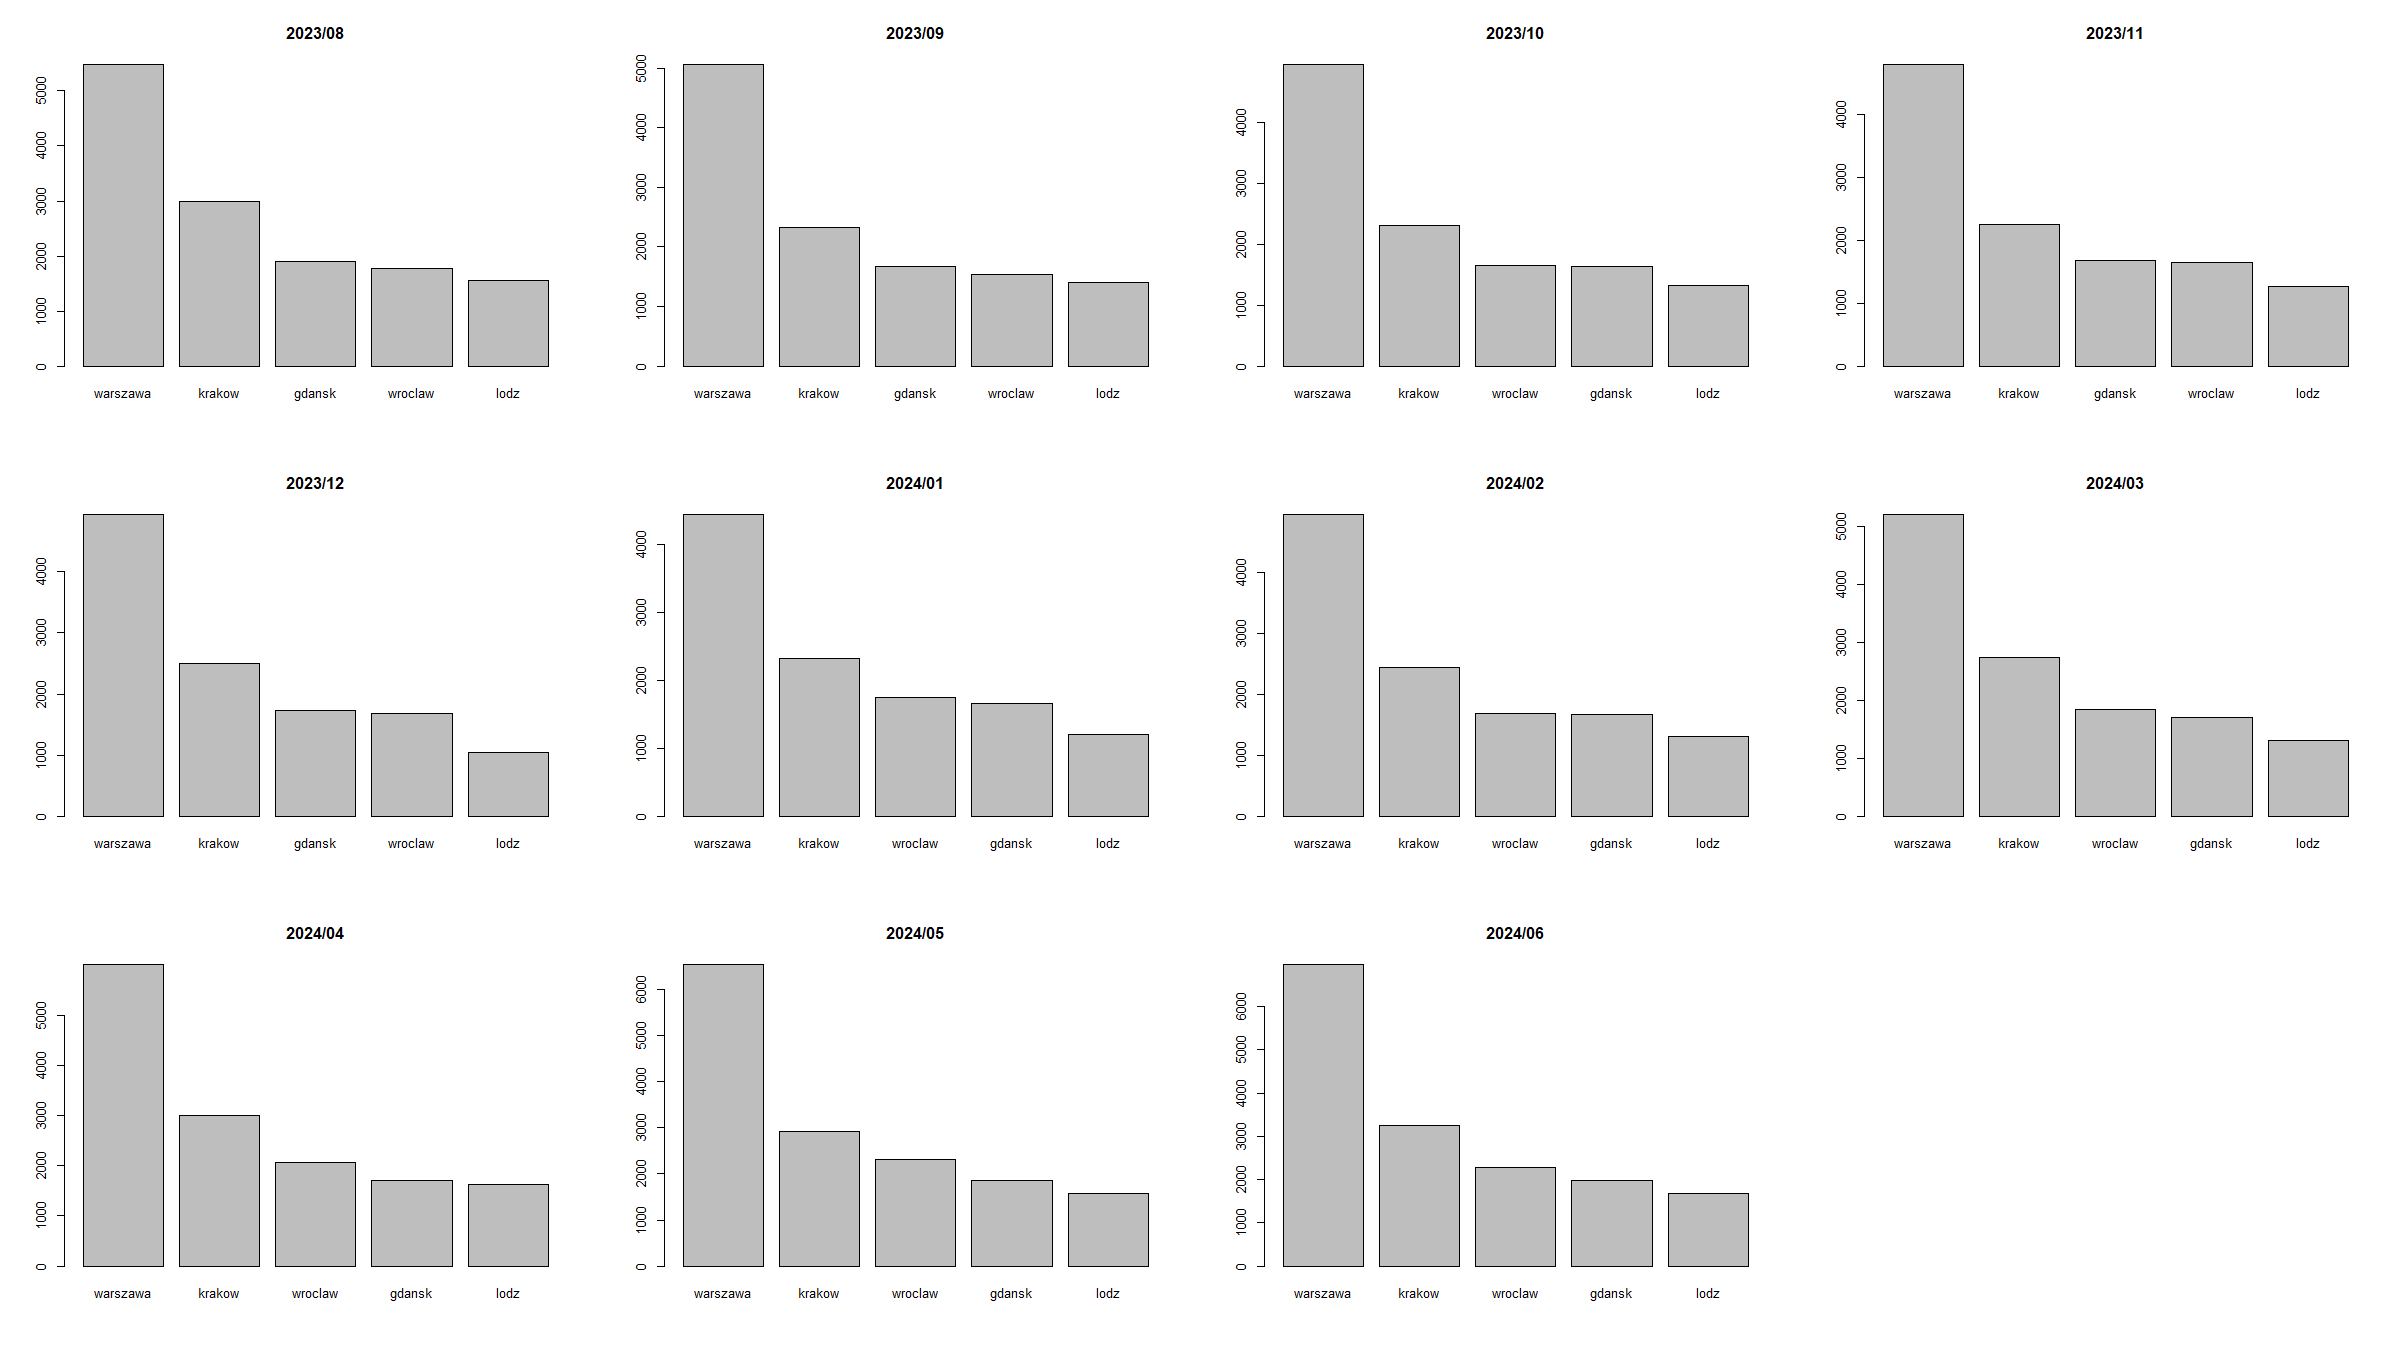
\includegraphics[width=0.99\linewidth]{miasta_najwiecej_wynajmow.png}
    \caption{Ilość wynajmów w poszczególnych miastach z podziałem na miesiące}
\end{figure}

Miastem, które wybraliśmy do analizy jest Kraków, który charakteryzuje się największą ilością wynajmów spośród wszystkich miast (oprócz Warszawy). Wybór ten pozwoli nam na uzyskanie bardziej reprezentatywnych wyników analizy skupień, ponieważ większa ilość danych umożliwi lepsze zidentyfikowanie wzorców i grup w danych dotyczących cen mieszkań w Krakowie.

\section{Cel i zakres badania}

\section{Przegląd literatury}

(min. 1 cytowanie powiązane tematycznie i krótki opis co było badane)

\section{Zmienne wybrane do analizy}

W analizie przyjęto podział zmiennych diagnostycznych na symulanty i destymulanty z punktu widzenia atrakcyjności mieszkania. Symulantami nazywa się cechy, których wyższe wartości są oceniane pozytywnie, natomiast destymulantami są cechy, których wzrost wpływa niekorzystnie na ocenę obiektu. Dobór zmiennych miał na celu uwzględnienie zarówno cech fizycznych mieszkania, jak i elementów związanych z jego lokalizacją oraz dostępnością infrastruktury w otoczeniu.

\medskip

Zmienne wybrane do analizy to:

\begin{enumerate}[leftmargin=*, label=\arabic*.]
    \item[] \textbf{Symulanty}

    \item \texttt{squareMeters} -- powierzchnia mieszkania wyrażona w metrach kwadratowych

    Zmienna ta opisuje wielkość lokalu mieszkalnego i należy do podstawowych cech charakteryzujących nieruchomość. Powierzchnia mieszkania wpływa bezpośrednio na komfort użytkowania, możliwości aranżacyjne oraz funkcjonalność przestrzeni. Większy metraż daje zazwyczaj większą swobodę zagospodarowania wnętrza i lepiej odpowiada na potrzeby gospodarstw domowych o większej liczbie członków. Z tego względu zmienna \texttt{squareMeters} została zakwalifikowana jako symulanta.

    \item \texttt{rooms} -- liczba pokoi w mieszkaniu

    Zmienna określa liczbę wydzielonych pomieszczeń mieszkalnych w lokalu, a więc w pewnym stopniu odzwierciedla jego układ funkcjonalny. Liczba pokoi ma istotne znaczenie z punktu widzenia użyteczności mieszkania, ponieważ wpływa na możliwość oddzielenia poszczególnych stref życia codziennego, takich jak wypoczynek, sen czy praca. Mieszkania z większą liczbą pokoi są często bardziej atrakcyjne dla rodzin oraz osób pracujących zdalnie. Dlatego zmienna \texttt{rooms} została uznana za symulantę.

    \item \texttt{poiCount} -- liczba punktów zainteresowania w promieniu 500 metrów od mieszkania

    Zmienna ta opisuje intensywność i dostępność infrastruktury w bezpośrednim otoczeniu nieruchomości. Obejmuje ona liczbę punktów zainteresowania znajdujących się w promieniu 500 metrów od mieszkania, takich jak sklepy, punkty usługowe, restauracje, placówki edukacyjne, przystanki komunikacji miejskiej czy inne obiekty użyteczności codziennej. Wyższa wartość tej zmiennej wskazuje na lepsze wyposażenie okolicy w usługi i udogodnienia, co zwiększa wygodę życia mieszkańców oraz atrakcyjność lokalizacji. W związku z tym \texttt{poiCount} została zakwalifikowana jako symulanta.

    \item \texttt{hasBalcony} -- informacja o obecności balkonu w mieszkaniu

    Zmienna ta ma charakter jakościowy i informuje, czy mieszkanie posiada balkon. Balkon stanowi dodatkową przestrzeń użytkową, która może pełnić funkcję rekreacyjną, wypoczynkową lub praktyczną. Obecność balkonu jest często postrzegana jako cecha podnosząca standard mieszkania, szczególnie w zabudowie wielorodzinnej. Na potrzeby analizy zmienna ta może zostać zakodowana binarnie, na przykład jako 1 dla odpowiedzi \texttt{yes} oraz 0 dla odpowiedzi \texttt{no}. Po takim przekształceniu wyższa wartość oznacza cechę bardziej pożądaną, dlatego \texttt{hasBalcony} potraktowano jako symulantę.

    \item[] \textbf{Destymulanty}

    \item \texttt{price} -- cena mieszkania

    Zmienna określa całkowitą cenę oferowanej nieruchomości i stanowi jedną z najważniejszych cech z punktu widzenia nabywcy. Cena wpływa bezpośrednio na dostępność ekonomiczną mieszkania oraz możliwość jego zakupu przez potencjalnych klientów. Przy porównywaniu mieszkań wyższa cena oznacza zwykle mniejszą dostępność finansową, nawet jeśli może częściowo wynikać z lepszej lokalizacji lub wyższego standardu. Z tego względu, w kontekście oceny atrakcyjności mieszkania z perspektywy ekonomicznej, zmienna \texttt{price} została uznana za destymulantę.

    \item \texttt{centreDistance} -- odległość mieszkania od centrum miasta w kilometrach

    Zmienna ta opisuje położenie nieruchomości względem centralnej części miasta. Lokalizacja jest jednym z kluczowych czynników wpływających na wartość i atrakcyjność mieszkania, ponieważ determinuje dostęp do miejsc pracy, usług, transportu publicznego, oferty handlowej i kulturalnej. W warunkach dużego miasta mniejsza odległość od centrum jest zazwyczaj postrzegana jako cecha korzystna, gdyż wiąże się z lepszą dostępnością najważniejszych funkcji miejskich. Wobec tego wzrost wartości zmiennej \texttt{centreDistance} obniża atrakcyjność nieruchomości, dlatego została ona zakwalifikowana jako destymulanta.

\end{enumerate}

\section{Wstępna analiza danych}

\subsection{Statystyki opisowe i podstawowa wizualizacja}

% (przynajmniej: średnia, mediana, minimum, maksimum, odchylenie standardowe, skośność)

\begin{table}[H]

\caption{Statystyki opisowe zmiennych wykorzystanych w analizie}
\centering
\begin{tabular}[t]{lrrrrrr}
\toprule
  & Srednia & Mediana & Minimum & Maksimum & OdchylenieStandardowe & Skosnosc\\
\midrule
price & 626 200.24 & 660 000.00 & 1 700.00 & 3 000 000.00 & 526 704.50 & 0.75\\
squareMeters & 55.35 & 50.49 & 25.00 & 150.00 & 21.38 & 1.48\\
rooms & 2.53 & 2.00 & 1.00 & 6.00 & 0.92 & 0.99\\
poiCount & 24.35 & 14.00 & 0.00 & 212.00 & 33.62 & 2.99\\
centreDistance & 3.82 & 3.71 & 0.14 & 9.99 & 2.17 & 0.38\\
hasBalcony & 0.63 & 1.00 & 0.00 & 1.00 & 0.48 & -0.55\\
\bottomrule
\end{tabular}
\end{table}

%np. boxplot, histogramy

% \begin{figure}[H]
%     \centering
%     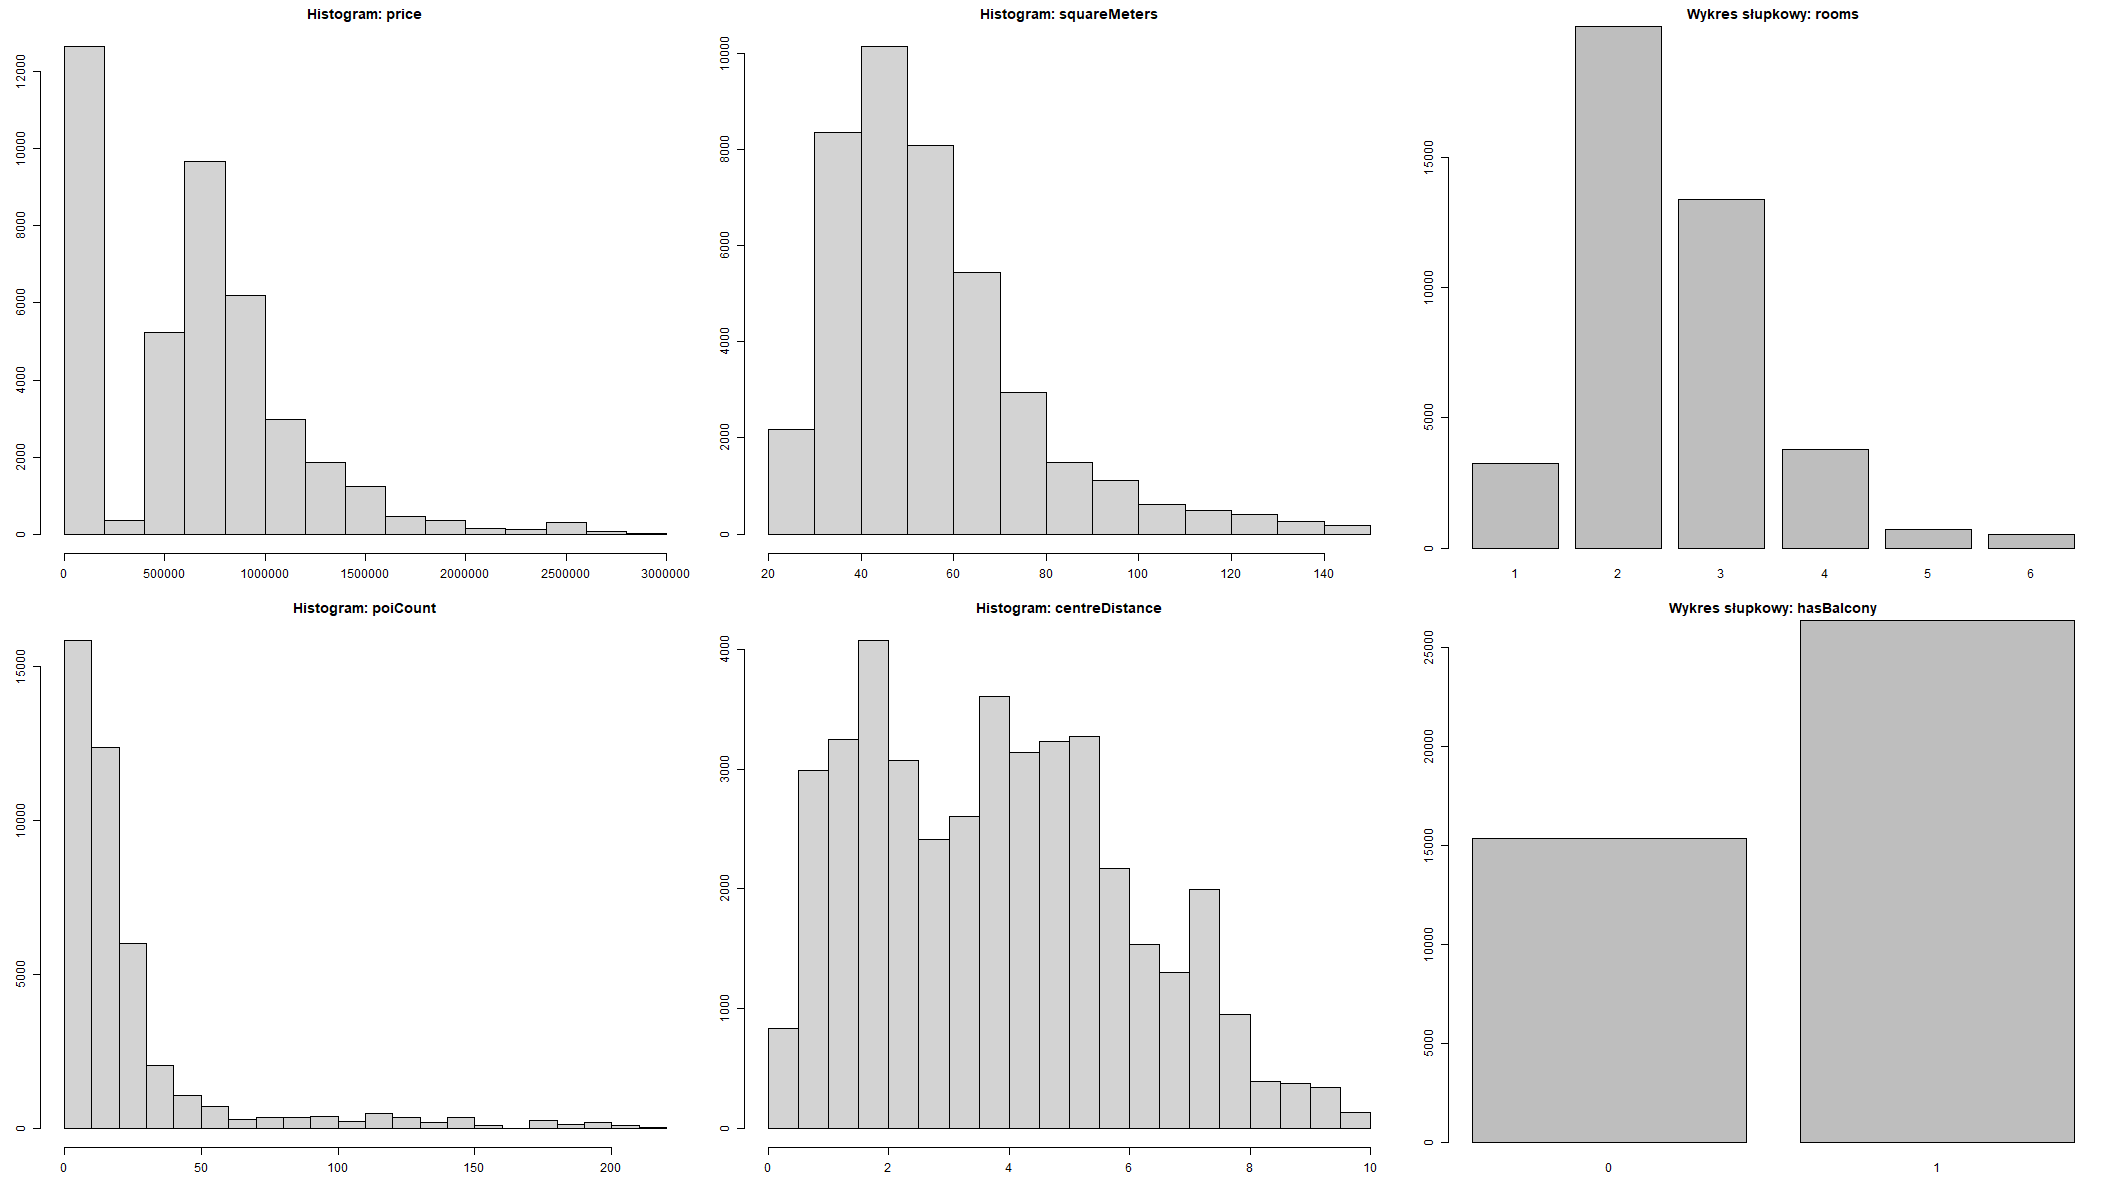
\includegraphics[width=0.99\linewidth]{Podstawowa_wizualizacja.png}
%     \caption{Wizualizacje}
% \end{figure}



\begin{figure}[H]
    \centering

    \begin{subfigure}[t]{0.48\linewidth}
        \centering
        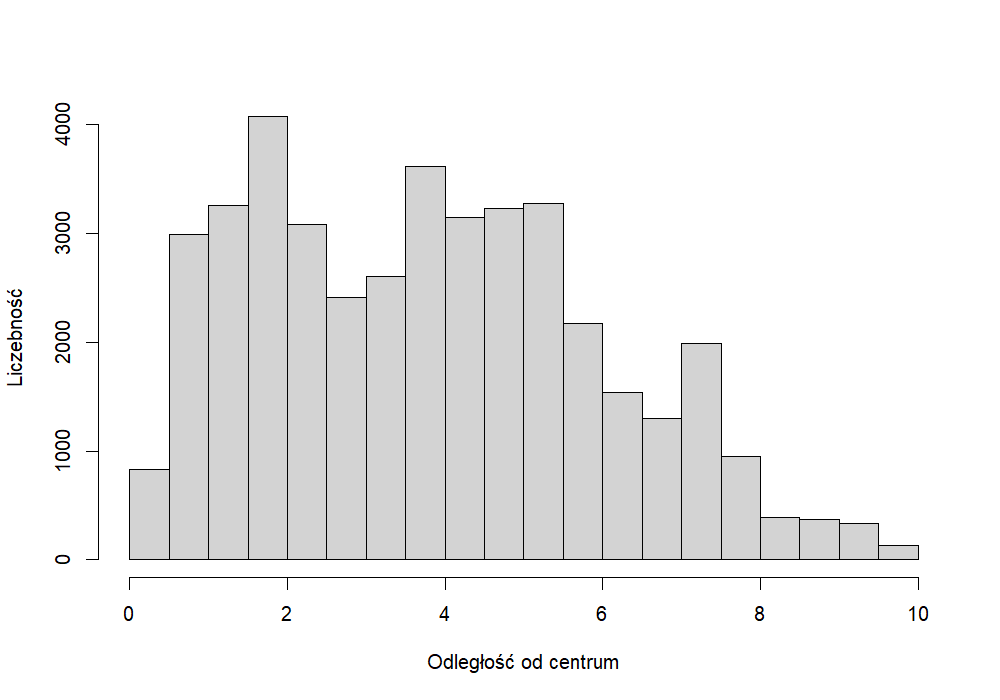
\includegraphics[width=\linewidth]{podstawowa_wizualizacja_centreDistance.png}
        \caption{Wizualizacja odległości mieszkań od centrum miasta}
    \end{subfigure}
    \hfill
    \begin{subfigure}[t]{0.48\linewidth}
        \centering
        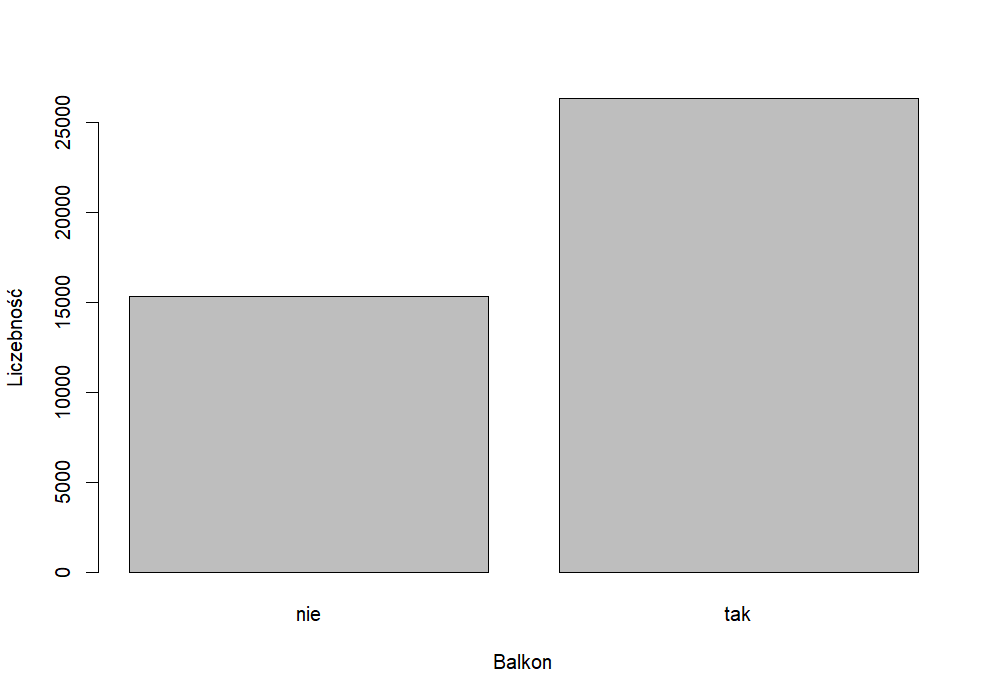
\includegraphics[width=\linewidth]{podstawowa_wizualizacja_hasBalcony.png}
        \caption{Wizualizacja ilości mieszkań z balkonem i bez balkonu}
    \end{subfigure}

    \vspace{0.5cm}

    \begin{subfigure}[t]{0.48\linewidth}
        \centering
        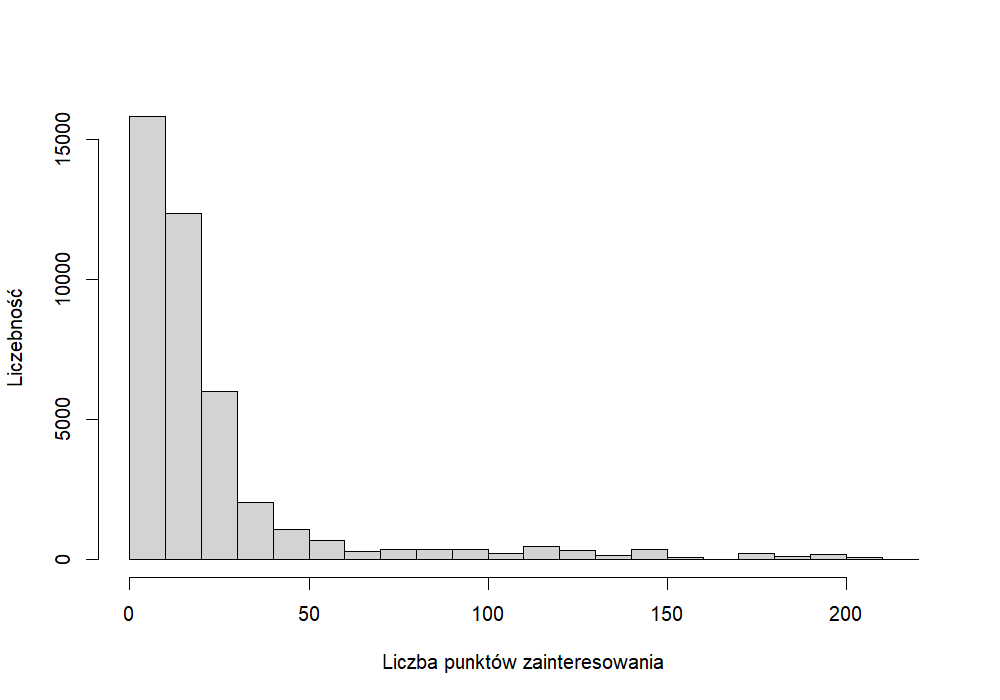
\includegraphics[width=\linewidth]{podstawowa_wizualizacja_poiCount.png}
        \caption{Wizualizacja ilości punktów zainteresowania w promieniu 500 metrów od mieszkań}
    \end{subfigure}
    \hfill
    \begin{subfigure}[t]{0.48\linewidth}
        \centering
        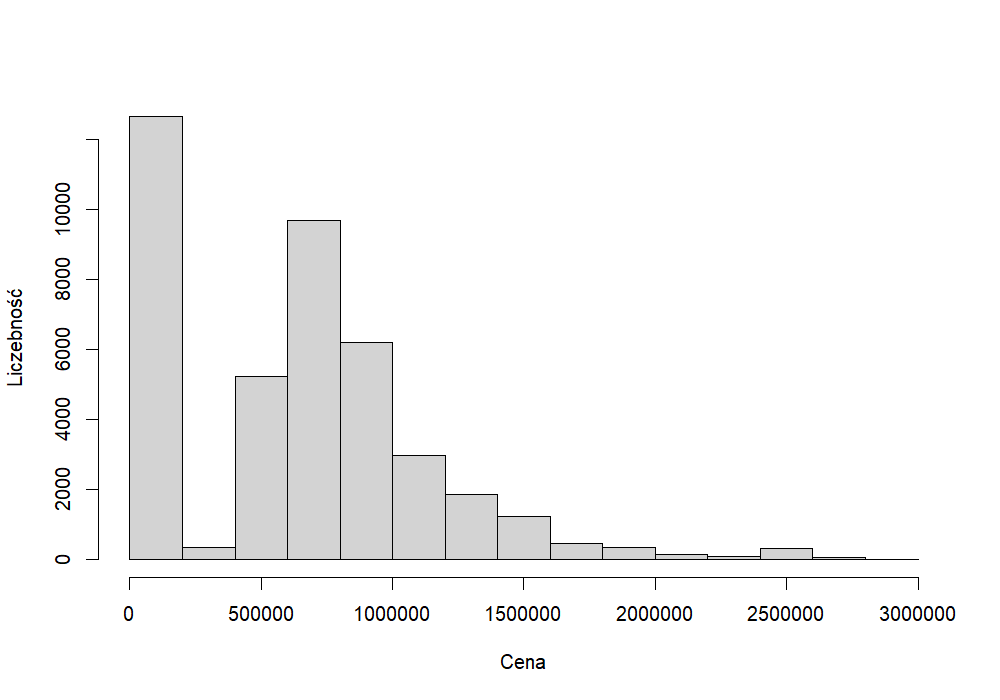
\includegraphics[width=\linewidth]{podstawowa_wizualizacja_price.png}
        \caption{Wizualizacja cen mieszkań}
    \end{subfigure}

    \vspace{0.5cm}

    \begin{subfigure}[t]{0.48\linewidth}
        \centering
        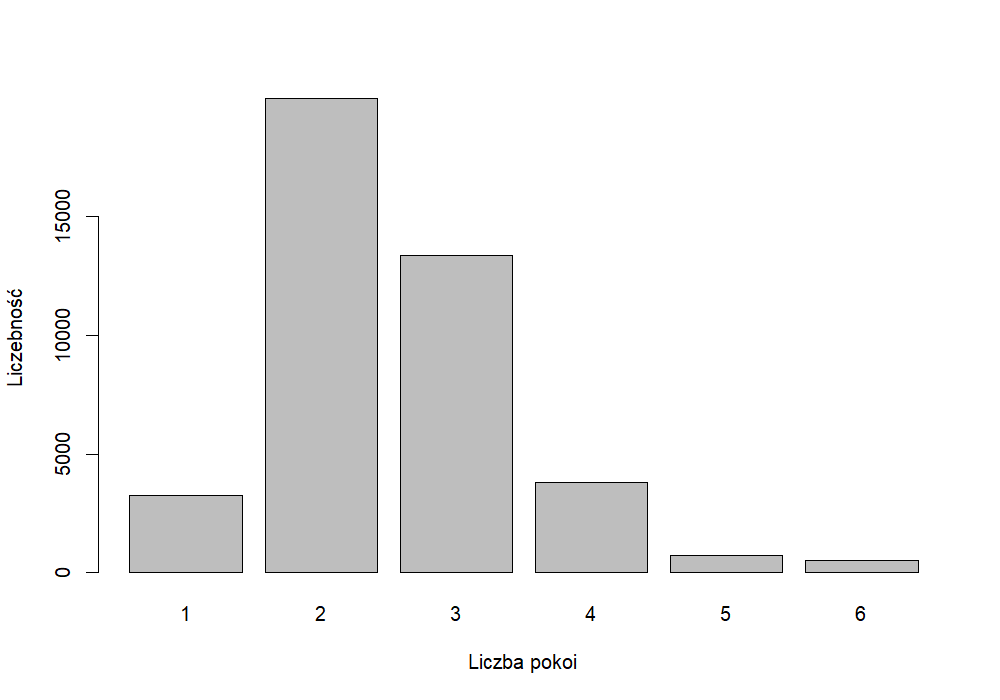
\includegraphics[width=\linewidth]{podstawowa_wizualizacja_rooms.png}
        \caption{Wizualizacja ilości pokoi w mieszkaniach}
    \end{subfigure}
    \hfill
    \begin{subfigure}[t]{0.48\linewidth}
        \centering
        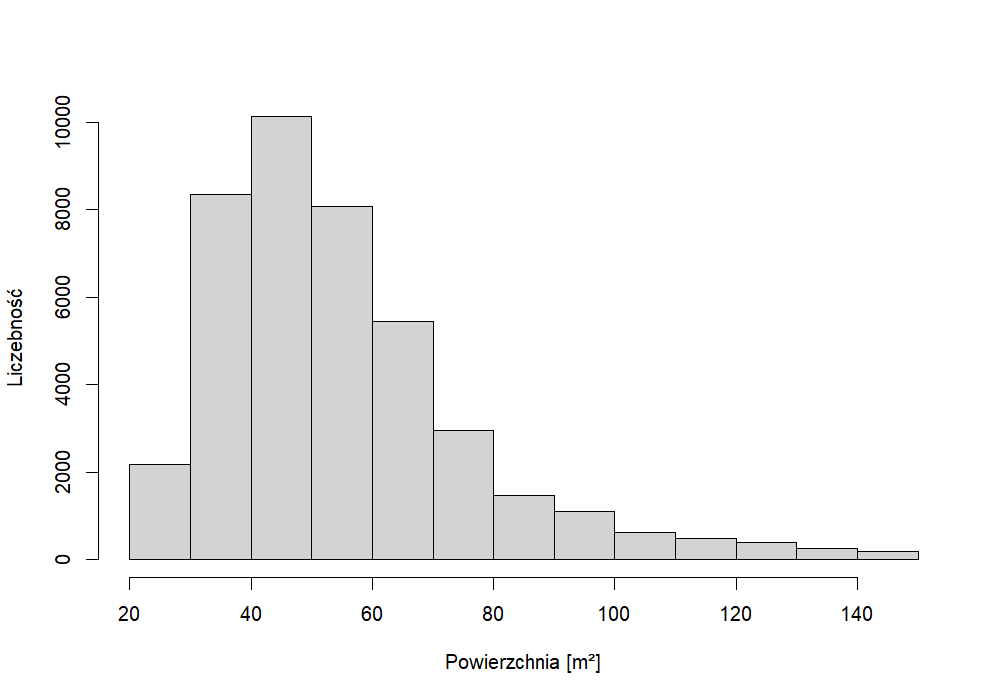
\includegraphics[width=\linewidth]{podstawowa_wizualizacja_squareMeters.png}
        \caption{Wizualizacja powierzchni mieszkań}
    \end{subfigure}

    \caption{Podstawowa wizualizacja zmiennych wykorzystanych w analizie}
\end{figure}

Statystyki opisowe oraz podstawowa wizualizacja zmiennych wykorzystanych w analizie umożliwiają ocenę struktury zbioru danych, rozkładu poszczególnych cech, stopnia ich zróżnicowania oraz ewentualnych nieregularności występujących w danych.

Rozkład zmiennej \texttt{price} oraz jej podstawowe charakterystyki statystyczne wskazują na obecność obserwacji należących do różnych segmentów rynku nieruchomości. Jest to związane z tym, że w zbiorze danych występują zarówno oferty mieszkań przeznaczonych na sprzedaż, jak i oferty mieszkań oferowanych na wynajem. Ze względu na brak bezpośredniej porównywalności cen najmu i cen sprzedaży, zakres dalszej analizy ograniczmy do ofert sprzedaży mieszkań.

Dokonujemy ponownych statystyk opisowych oraz wizualizacji, uwzględniając tylko oferty sprzedaży mieszkań. Dzięki temu uzyskamy bardziej spójny i porównywalny zbiór danych, który pozwoli na rzetelną analizę skupień oraz identyfikację grup podobnych ofert w kontekście cen mieszkań przeznaczonych na sprzedaż.

\begin{table}[H]

\caption{Statystyki opisowe zmiennych wykorzystanych w analizie po usunięciu ofert wynajmu mieszkań}
\centering
\begin{tabular}[t]{lrrrrrr}
\toprule
  & Srednia & Mediana & Minimum & Maksimum & OdchylenieStandardowe & Skosnosc\\
\midrule
price & 897 888.77 & 795 000.00 & 255 000.00 & 3 000 000.00 & 394 185.67 & 1.89\\
squareMeters & 57.17 & 52.00 & 25.00 & 150.00 & 22.12 & 1.43\\
rooms & 2.63 & 3.00 & 1.00 & 6.00 & 0.95 & 0.91\\
poiCount & 23.94 & 14.00 & 0.00 & 212.00 & 33.80 & 3.07\\
centreDistance & 4.01 & 3.95 & 0.15 & 9.99 & 2.21 & 0.28\\
hasBalcony & 0.62 & 1.00 & 0.00 & 1.00 & 0.49 & -0.49\\
\bottomrule
\end{tabular}
\end{table}

\begin{figure}[H]
    \centering

    \begin{subfigure}[t]{0.48\linewidth}
        \centering
        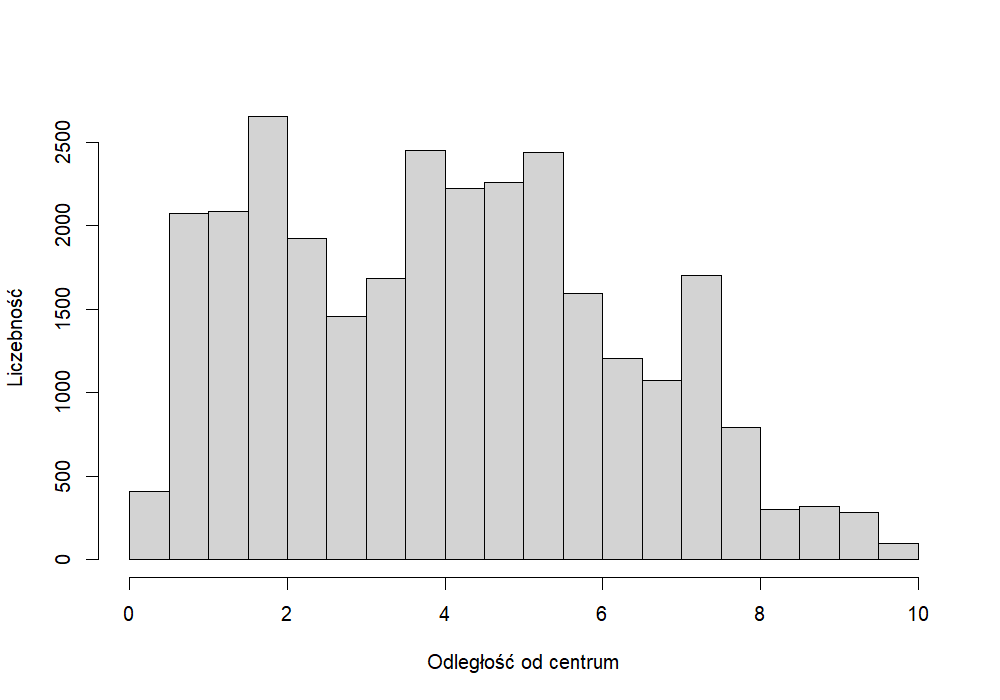
\includegraphics[width=\linewidth]{podstawowa_wizualizacja_centreDistance_sama_sprzedaz.png}
        \caption{Wizualizacja odległości mieszkań od centrum miasta}
    \end{subfigure}
    \hfill
    \begin{subfigure}[t]{0.48\linewidth}
        \centering
        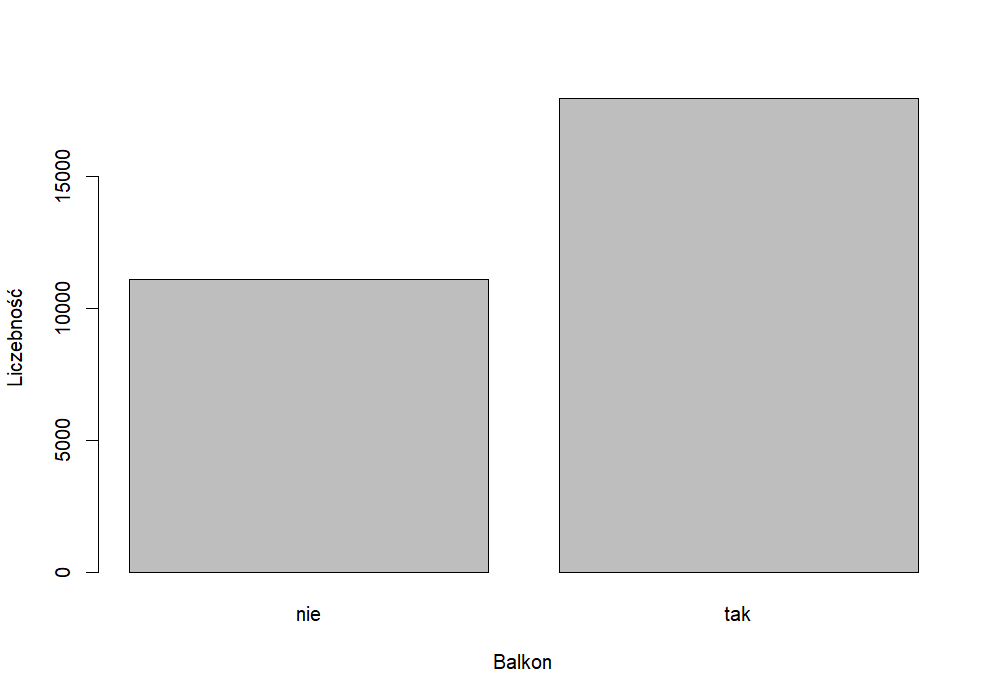
\includegraphics[width=\linewidth]{podstawowa_wizualizacja_hasBalcony_sama_sprzedaz.png}
        \caption{Wizualizacja ilości mieszkań z balkonem i bez balkonu}
    \end{subfigure}

    \vspace{0.5cm}

    \begin{subfigure}[t]{0.48\linewidth}
        \centering
        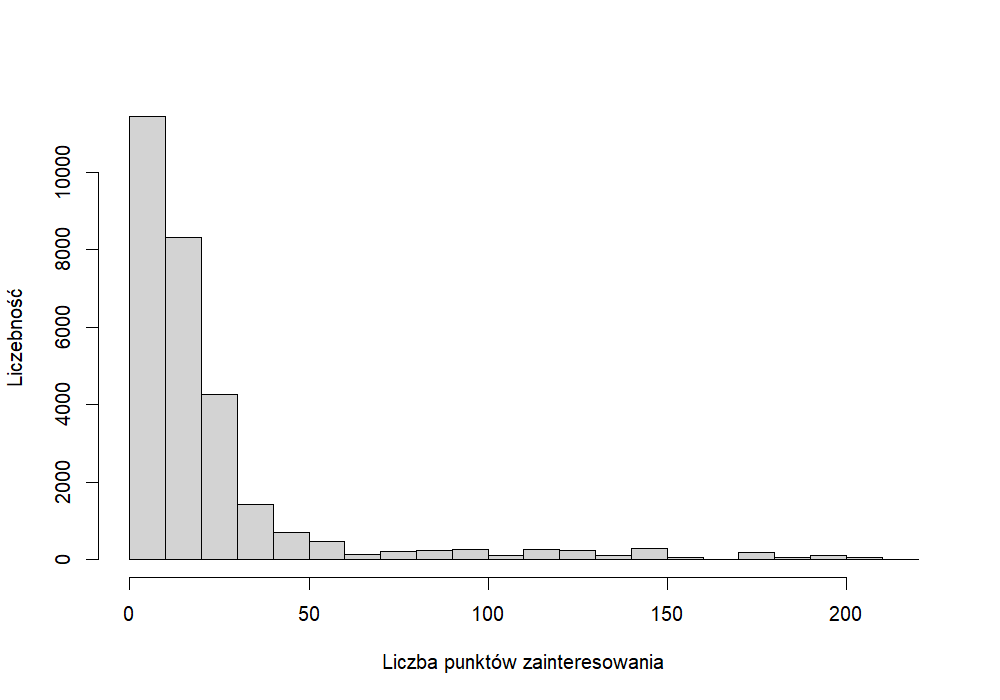
\includegraphics[width=\linewidth]{podstawowa_wizualizacja_poiCount_sama_sprzedaz.png}
        \caption{Wizualizacja ilości punktów zainteresowania w promieniu 500 metrów od mieszkań}
    \end{subfigure}
    \hfill
    \begin{subfigure}[t]{0.48\linewidth}
        \centering
        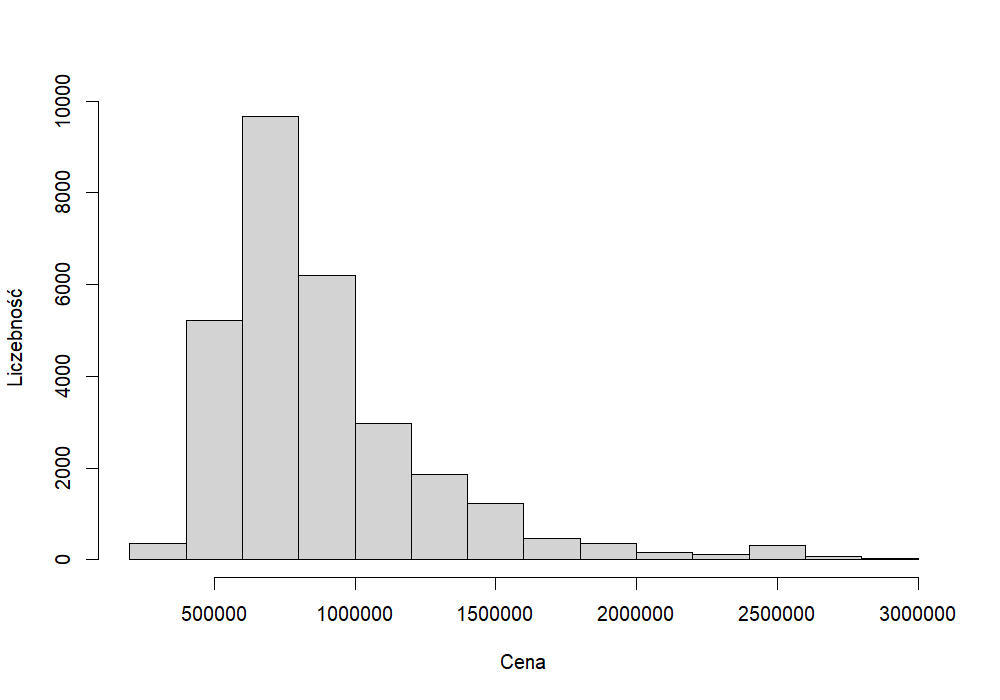
\includegraphics[width=\linewidth]{podstawowa_wizualizacja_price_sama_sprzedaz.png}
        \caption{Wizualizacja cen mieszkań}
    \end{subfigure}

    \vspace{0.5cm}

    \begin{subfigure}[t]{0.48\linewidth}
        \centering
        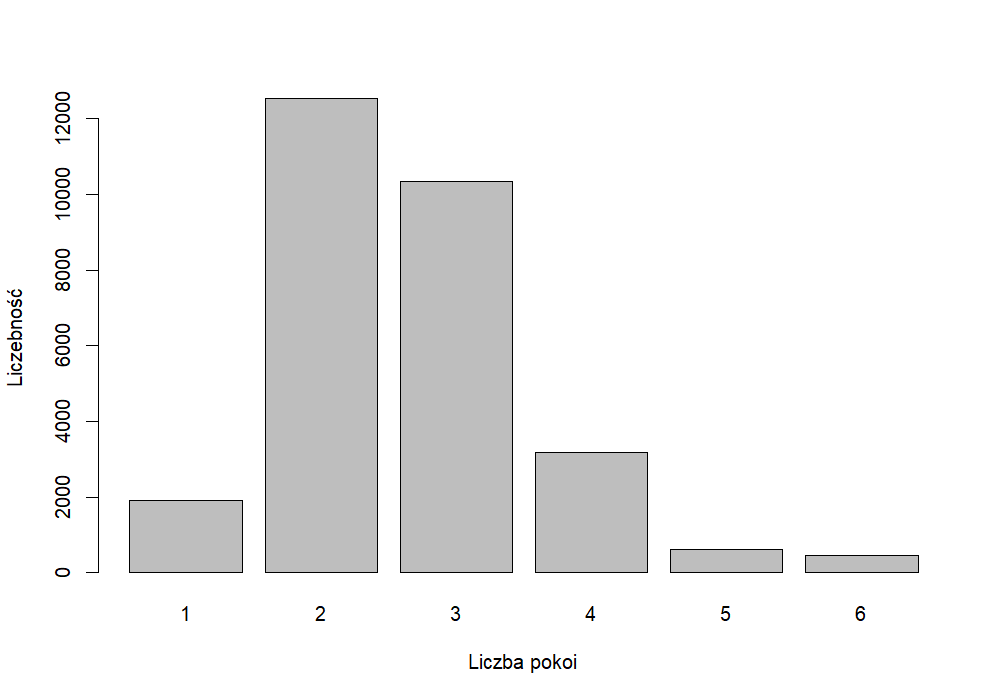
\includegraphics[width=\linewidth]{podstawowa_wizualizacja_rooms_sama_sprzedaz.png}
        \caption{Wizualizacja ilości pokoi w mieszkaniach}
    \end{subfigure}
    \hfill
    \begin{subfigure}[t]{0.48\linewidth}
        \centering
        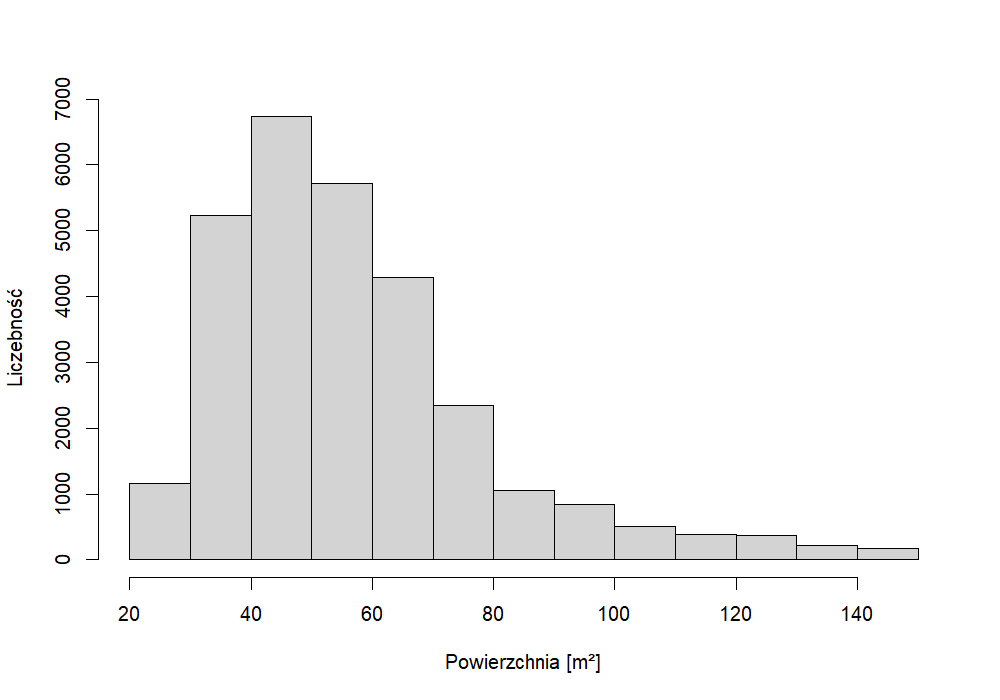
\includegraphics[width=\linewidth]{podstawowa_wizualizacja_squareMeters_sama_sprzedaz.png}
        \caption{Wizualizacja powierzchni mieszkań}
    \end{subfigure}

    \caption{Podstawowa wizualizacja zmiennych wykorzystanych w analizie po usunięciu ofert wynajmu mieszkań.}
\end{figure}



% \subsection{Standaryzacja danych}


% W toku wstępnej analizy zbioru danych zauważono, że zmienna \texttt{price} nie była zapisana w jednolity sposób dla wszystkich obserwacji. Część ofert zawierała cenę całkowitą mieszkania, natomiast w przypadku części ogłoszeń cena była wyrażona jako cena za metr kwadratowy. Taka niejednorodność zapisu prowadzi do braku porównywalności obserwacji i może istotnie zaburzać wyniki dalszej analizy statystycznej oraz analizy skupień.

% Przesłanką wskazującą na występowanie dwóch różnych sposobów zapisu ceny był wyraźny uskok w rozkładzie wartości zmiennej \texttt{price}, widoczny pomiędzy poziomem około 10\,000 a 255\,000. Wartości z dolnego zakresu odpowiadają realistycznym cenom za metr kwadratowy mieszkania, natomiast wartości wyraźnie wyższe interpretowano jako ceny całkowite nieruchomości. Taki rozkład sugerował, że w zbiorze jednocześnie występują dwie różne jednostki opisu tej samej cechy.

% \begin{figure}[H]
%     \centering
%     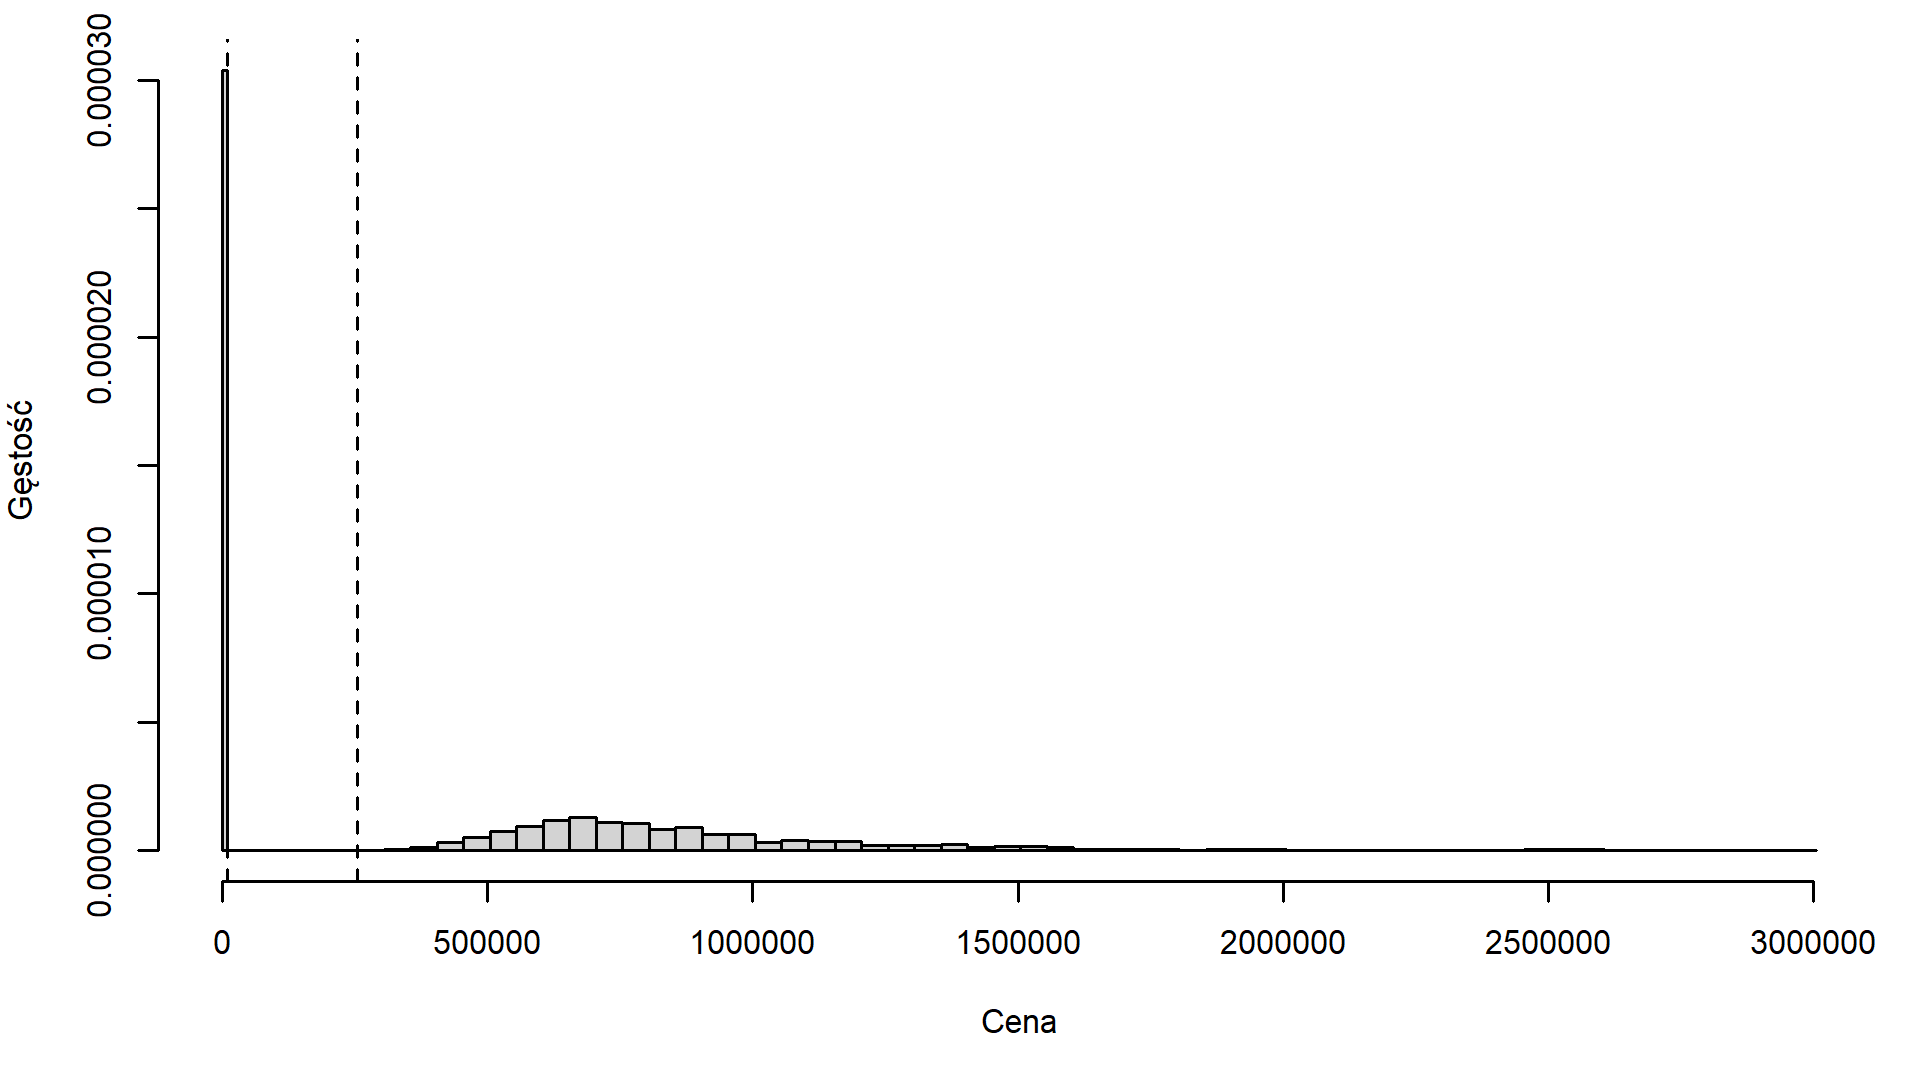
\includegraphics[width=0.99\linewidth]{histogram_price_z_uskokiem.png}
%     \caption{Dokładna wizualizacja rozkładu zmiennej \texttt{price} z zaznaczeniem uskoku wskazującego na niejednorodność zapisu cen.}
% \end{figure}


% \begin{table}[H]
% \centering
% \begin{tabular}[t]{lrrrrrr}
% \toprule
%   & price & squareMeters & rooms & poiCount & centreDistance & hasBalcony\\
% \midrule
% \multicolumn{7}{c}{\dots}\\
% 213569 & 10 000 & 108.00 & 4 & 19 & 1.64 & 0\\
% 213620 & 10 000 & 108.00 & 4 & 19 & 1.78 & 1\\
% 214046 & 10 000 & 107.74 & 5 & 21 & 1.24 & 0\\
% 214181 & 10 000 & 110.00 & 5 & 19 & 1.28 & 1\\
% 214699 & 10 000 & 100.00 & 4 & 66 & 1.40 & 1\\
% 214804 & 10 000 & 135.00 & 4 & 72 & 1.04 & 1\\
% %\addlinespace
% 3336 & 255 000 & 37.20 & 2 & 6 & 4.13 & 0\\
% 37236 & 255 129 & 32.94 & 2 & 24 & 7.27 & 0\\
% 3782 & 266 000 & 35.50 & 2 & 9 & 4.06 & 0\\
% 20941 & 280 000 & 29.00 & 2 & 18 & 6.71 & 0\\
% 55548 & 282 000 & 41.00 & 2 & 3 & 5.44 & 1\\
% \multicolumn{7}{c}{\dots}\\
% \bottomrule
% \end{tabular}
% \caption{Obserwacje bezpośrednio przed i po uskoku w rozkładzie zmiennej \texttt{price}, ilustrujące różnicę w zapisie cen mieszkań.}
% \end{table}

% W celu ujednolicenia danych zdecydowano się na sprowadzenie wszystkich obserwacji do wspólnej postaci, to znaczy do \textbf{ceny za metr kwadratowy}. Dla obserwacji, w których cena była zapisana jako cena całkowita mieszkania, dokonano przeliczenia przez podzielenie wartości zmiennej \texttt{price} przez zmienną \texttt{squareMeters}. Obserwacje, których wartości wskazywały na to, że cena była już wyrażona w przeliczeniu na metr kwadratowy, pozostawiono bez zmian.

% Przyjęte podejście pozwoliło na usunięcie niejednorodności jednostek pomiaru i zapewniło porównywalność danych w dalszych etapach analizy. Jest to szczególnie istotne w analizie skupień, w której odległości pomiędzy obiektami są wyznaczane bezpośrednio na podstawie wartości zmiennych. Pozostawienie zmiennej \texttt{price} w niejednolitym formacie mogłoby prowadzić do sztucznego różnicowania mieszkań wyłącznie z powodu odmiennego sposobu zapisu ceny, a nie rzeczywistych różnic pomiędzy nieruchomościami.


% \begin{figure}[H]
%     \centering
%     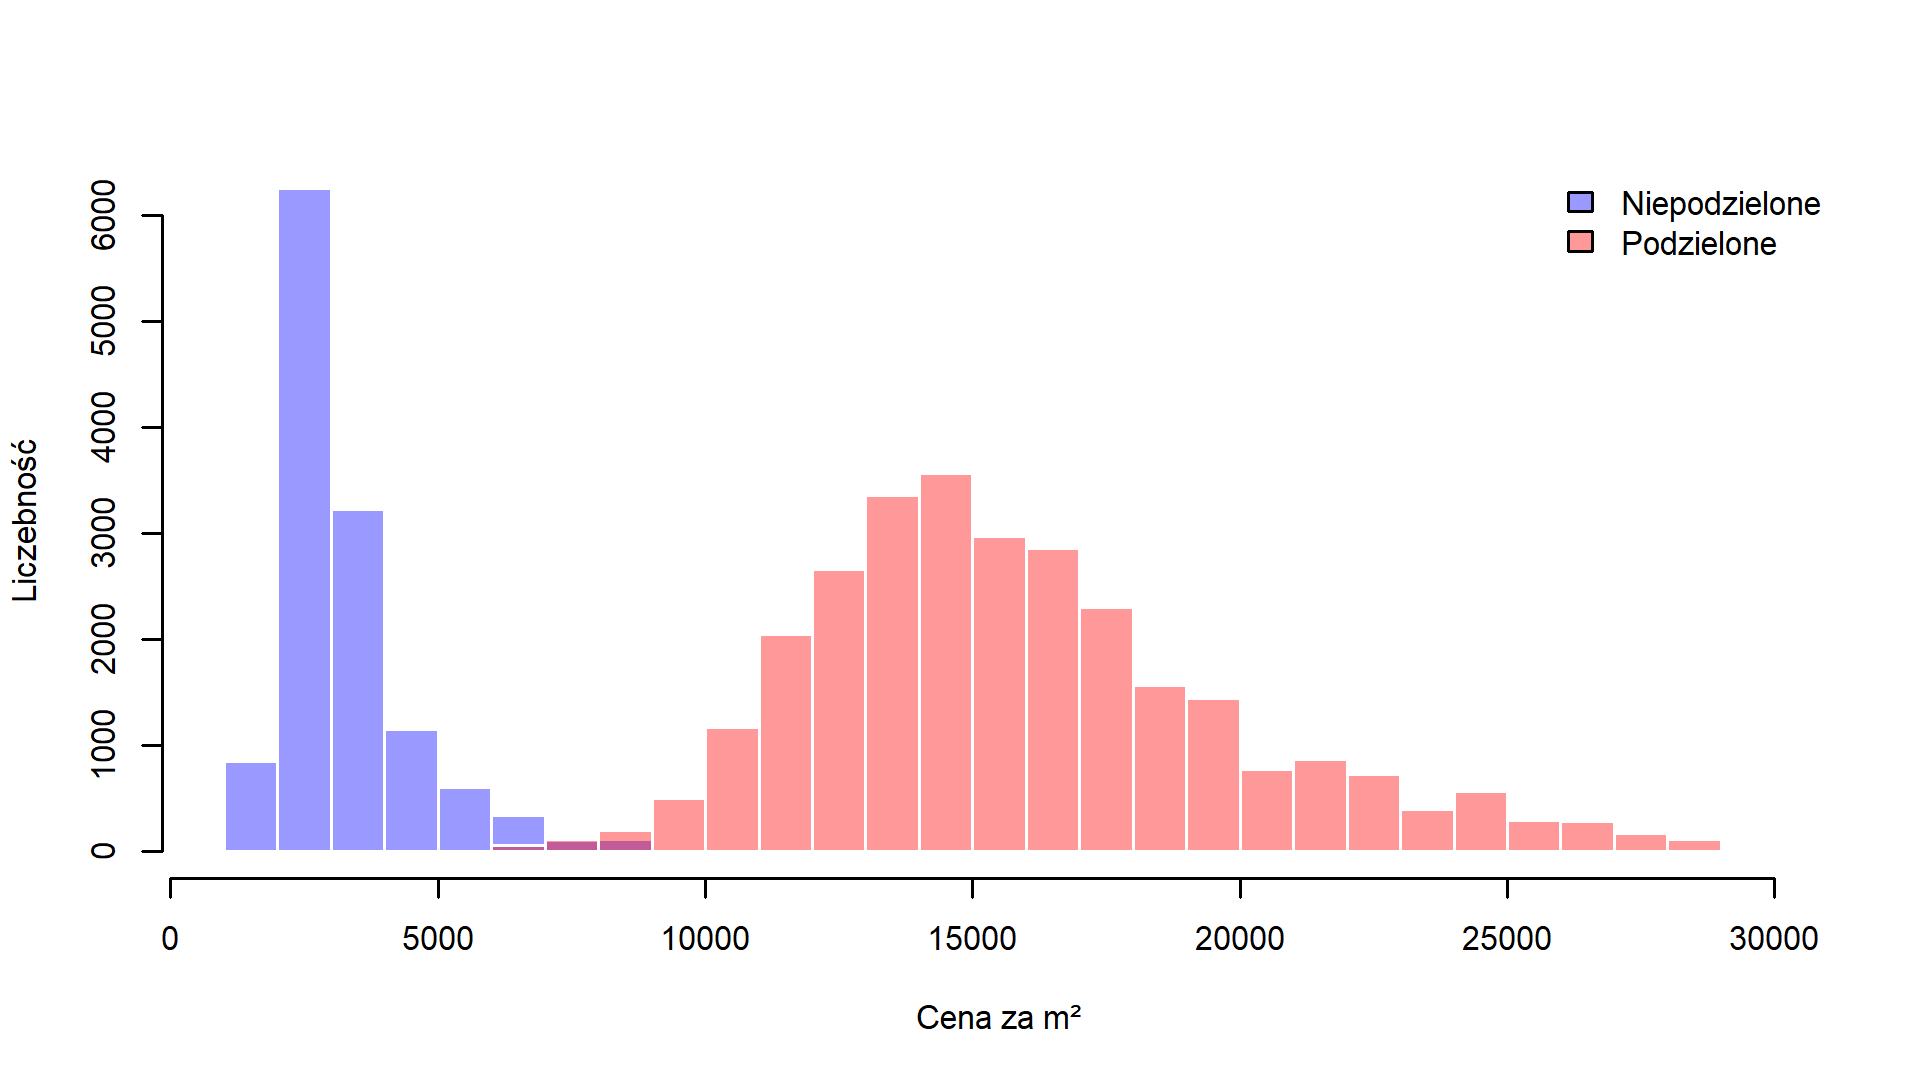
\includegraphics[width=0.99\linewidth]{histogram_price_z_podzialem.png}
%     \caption{}
% \end{figure}


\subsection{braki danych}

% czy występują i jak je obsłużono

Ocena kompletności danych stanowi istotny element wstępnej analizy zbioru, ponieważ obecność brakujących wartości może wpływać na wiarygodność wyników oraz ograniczać możliwość zastosowania wybranych metod statystycznych. Z tego względu sprawdzeniu poddano wszystkie zmienne uwzględnione w dalszej analizie, tj. \texttt{price}, \texttt{squareMeters}, \texttt{rooms}, \texttt{poiCount}, \texttt{centreDistance} oraz \texttt{hasBalcony}.

W analizowanych danych nie występują braki wartości dla żadnej z uwzględnionych zmiennych. Każda obserwacja zawiera zatem pełny zestaw informacji wymaganych w dalszych etapach badania. Dzięki temu dalsza analiza nie wymaga ani uzupełniania danych, ani ograniczania zbioru do obserwacji kompletnych.

\subsection{Obserwacje odstające}

Analiza obserwacji odstających (ang. \textit{outliers}) jest kluczowym etapem przygotowania zbioru danych, ponieważ algorytmy analizy skupień są szczególnie wrażliwe na wartości ekstremalne. Mogą one prowadzić do błędnej interpretacji wyników, przesuwając środki ciężkości tworzonych grup lub tworząc sztuczne, mało liczebne skupiska.

Wartości odstające zidentyfikowano przy użyciu metody rozstępu międzykwartylowego (IQR), definiując obserwacje jako odstające, jeśli znajdowały się poza przedziałem \([Q1 - 1.5 \cdot IQR,\; Q3 + 1.5 \cdot IQR]\). Proces czyszczenia danych skupił się na następujących aspektach:

\begin{itemize}
    \item \textbf{Cena i powierzchnia:} Usunięto oferty, w których cena lub metraż przyjmowały wartości nierealne z punktu widzenia rynku nieruchomości (np. mieszkania o powierzchni powyżej 200 $m^2$ lub ceny jednostkowe drastycznie odbiegające od średniej rynkowej dla Krakowa). Wartości te mogły wynikać z błędów przy wprowadzaniu ogłoszeń.
    \item \textbf{Liczba pokoi:} Zweryfikowano rekordy, w których liczba pokoi była nieproporcjonalna do metrażu. Skupiono się na standardowych lokalach mieszkalnych, eliminując skrajne przypadki, które mogłyby zaburzyć strukturę budowanych skupień.
    \item \textbf{Dystans od centrum:} Sprawdzono poprawność zmiennej \texttt{centreDistance}, aby wykluczyć błędy w lokalizacji, które mogłyby sugerować położenie nieruchomości poza granicami badanego obszaru.
\end{itemize}
W wyniku zastosowanej procedury czyszczenia danych liczba obserwacji została zredukowana z 29\,026 do 24\,353, co stanowi około 83.9\% pierwotnego zbioru danych. Oznacza to, że usunięto około 16.1\% rekordów jako zawierających wartości odstające w co najmniej jednej z analizowanych zmiennych.

Ostatecznie, po usunięciu najbardziej skrajnych obserwacji, zbiór danych stał się bardziej spójny. Pozwoliło to na uzyskanie stabilniejszych wyników w dalszych etapach modelowania, zapewniając, że wyodrębnione skupienia będą reprezentować rzeczywiste segmenty rynku, a nie błędy w danych lub przypadki jednostkowe.



\begin{table}[H]

\caption{Statystyki opisowe po usunięciu obserwacji odstających}
\centering
\begin{tabular}[t]{lrrrrrr}
\toprule
  & Srednia & Mediana & Minimum & Maksimum & OdchylenieStandardowe & Skosnosc\\
\midrule
price & 802 044.61 & 750 000.00 & 255 000.00 & 1 649 000.00 & 250 133.54 & 0.90\\
squareMeters & 52.56 & 50.75 & 25.00 & 102.72 & 15.35 & 0.63\\
rooms & 2.48 & 2.00 & 1.00 & 4.00 & 0.76 & 0.18\\
poiCount & 14.16 & 12.00 & 0.00 & 49.00 & 10.39 & 0.88\\
centreDistance & 4.42 & 4.36 & 0.42 & 9.99 & 2.06 & 0.25\\
\addlinespace
hasBalcony & 0.64 & 1.00 & 0.00 & 1.00 & 0.48 & -0.60\\
\bottomrule
\end{tabular}
\end{table}

\begin{figure}[H]
\centering

\begin{minipage}{0.48\textwidth}
    \centering
    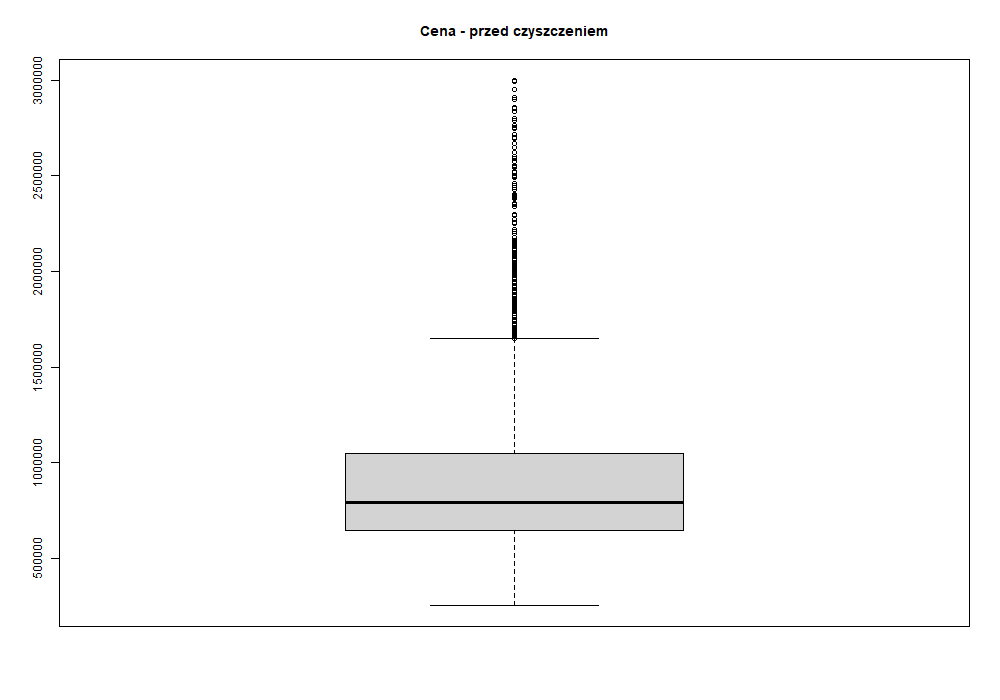
\includegraphics[width=\textwidth]{boxplot_price.png}
    \caption{Cena mieszkań przed czyszczeniem}
\end{minipage}
\hfill
\begin{minipage}{0.48\textwidth}
    \centering
    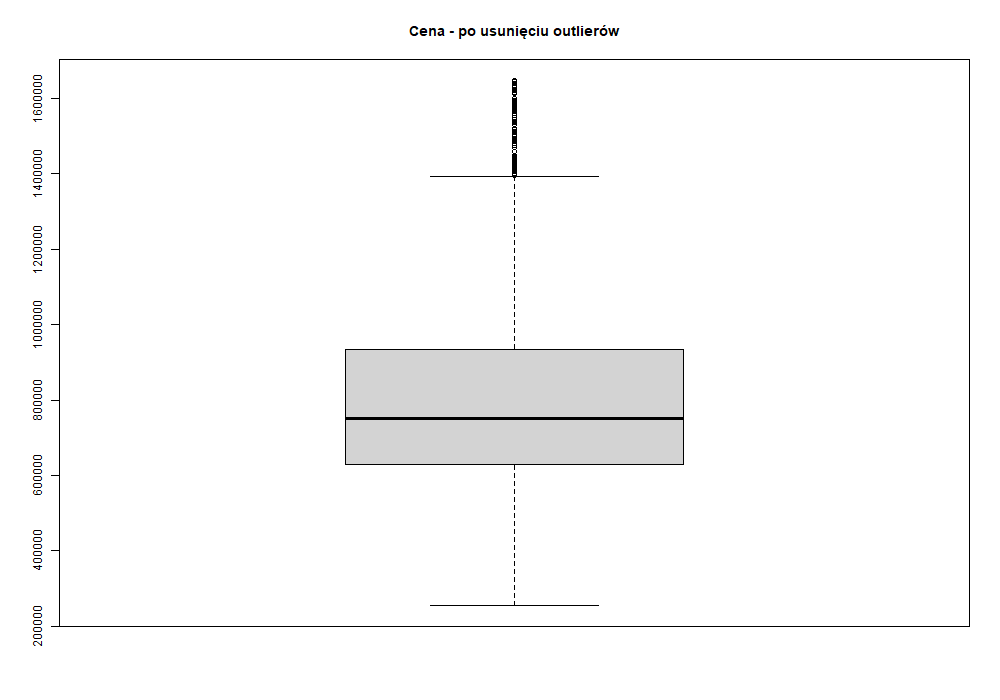
\includegraphics[width=\textwidth]{boxplot_price_clean.png}
    \caption{Cena mieszkań po czyszczeniu}
\end{minipage}

\vspace{0.5cm}

\begin{minipage}{0.48\textwidth}
    \centering
    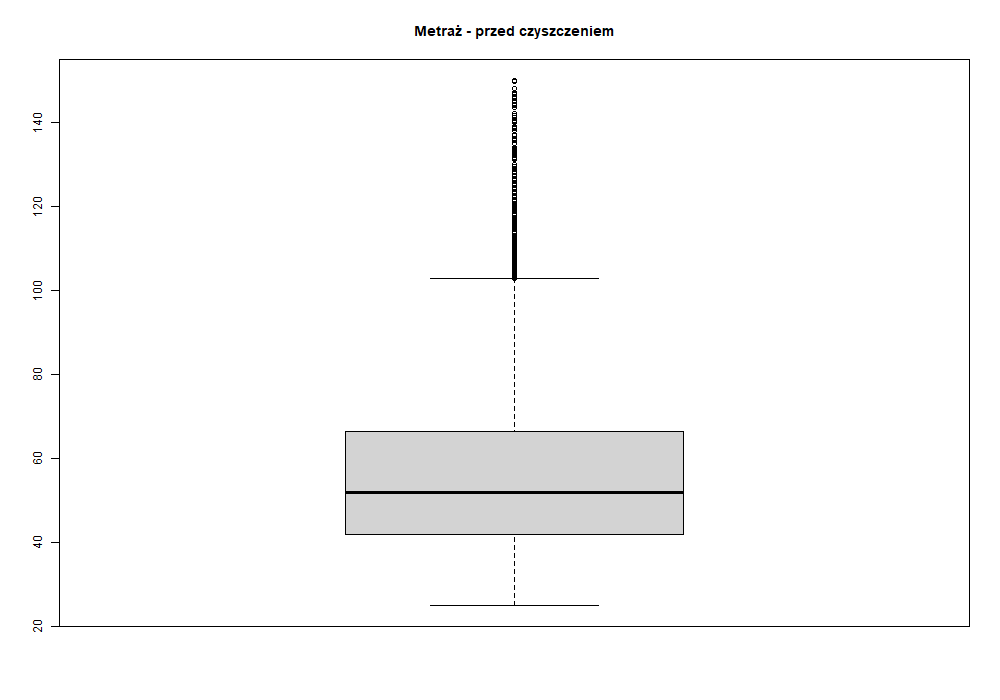
\includegraphics[width=\textwidth]{boxplot_squareMeters.png}
    \caption{Metraż przed czyszczeniem}
\end{minipage}
\hfill
\begin{minipage}{0.48\textwidth}
    \centering
    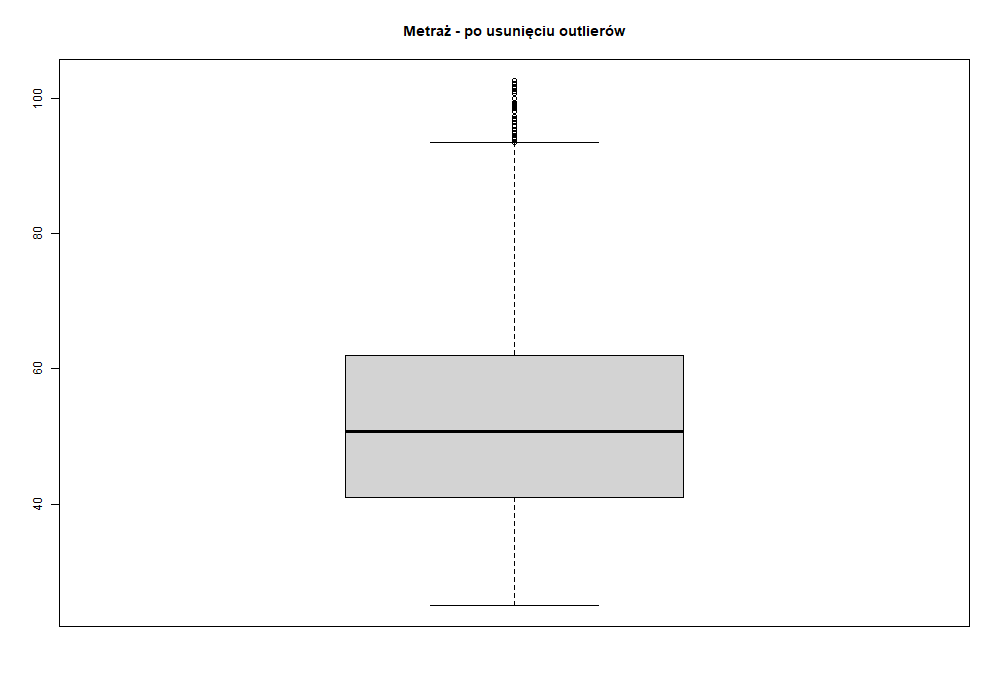
\includegraphics[width=\textwidth]{boxplot_squareMeters_clean.png}
    \caption{Metraż po czyszczeniu}
\end{minipage}

\vspace{0.5cm}

\begin{minipage}{0.48\textwidth}
    \centering
    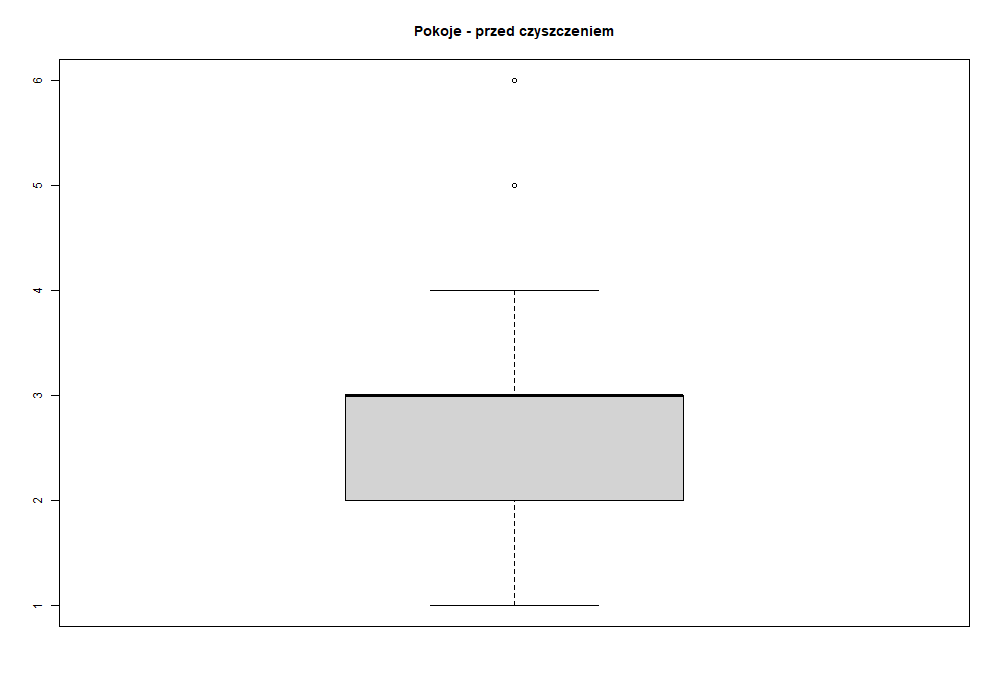
\includegraphics[width=\textwidth]{boxplot_rooms.png}
    \caption{Pokoje przed czyszczeniem}
\end{minipage}
\hfill
\begin{minipage}{0.48\textwidth}
    \centering
    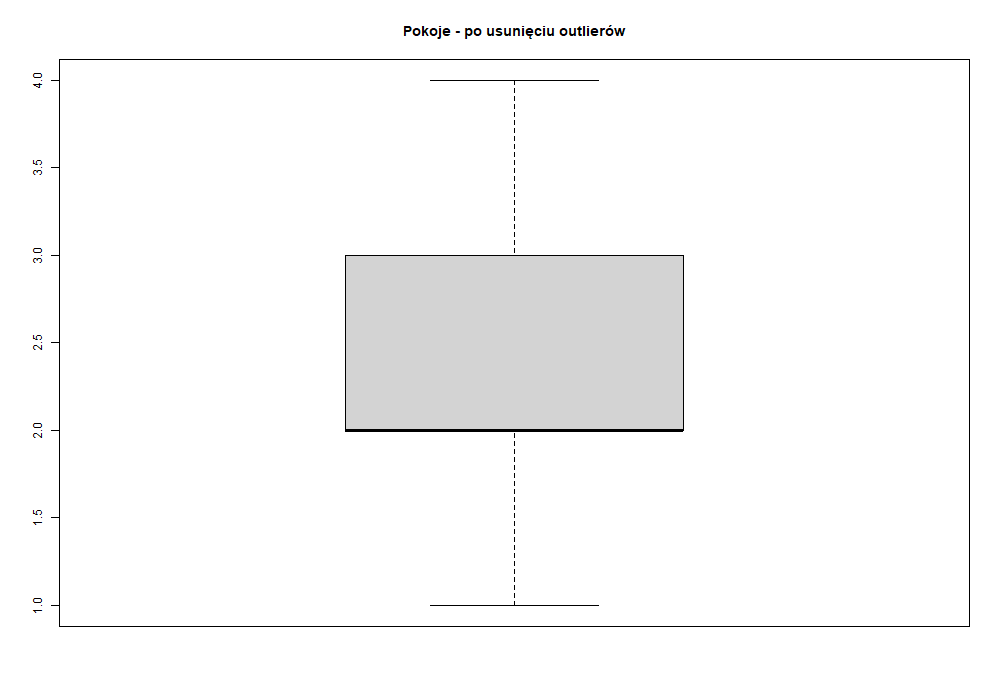
\includegraphics[width=\textwidth]{boxplot_rooms_clean.png}
    \caption{Pokoje po czyszczeniu}
\end{minipage}

\end{figure}


\begin{figure}[H]
\centering

\begin{minipage}{0.48\textwidth}
    \centering
    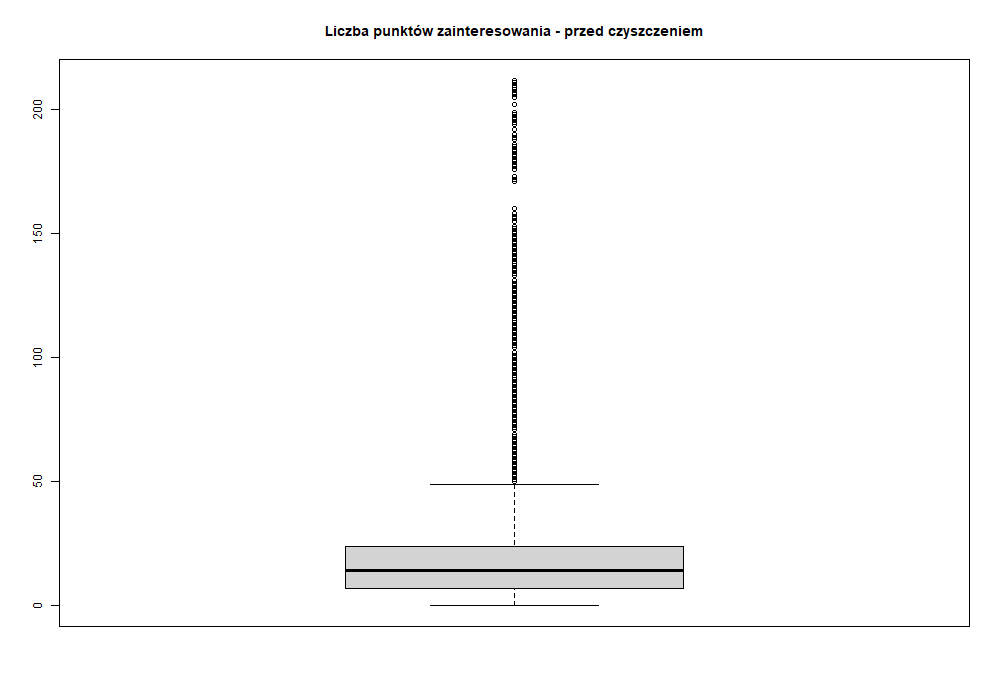
\includegraphics[width=\textwidth]{boxplot_poiCount.png}
    \caption{Liczba punktów zainteresowania przed czyszczeniem}
\end{minipage}
\hfill
\begin{minipage}{0.48\textwidth}
    \centering
    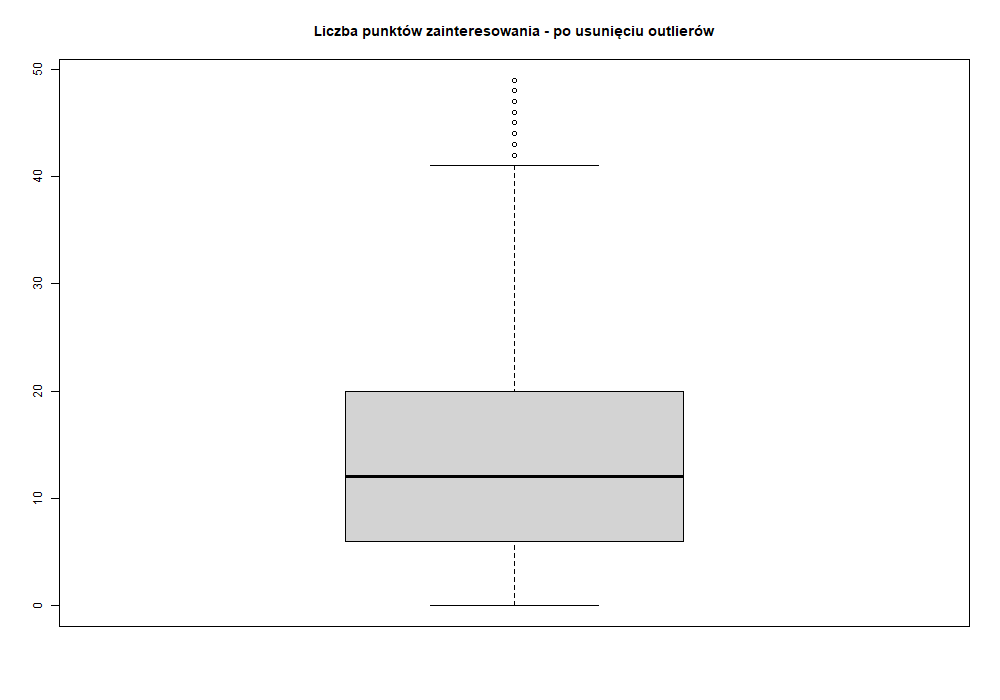
\includegraphics[width=\textwidth]{boxplot_poiCoint_clean.png}
    \caption{Liczba punktów zainteresowania po czyszczeniu}
\end{minipage}

\vspace{0.5cm}

\begin{minipage}{0.48\textwidth}
    \centering
    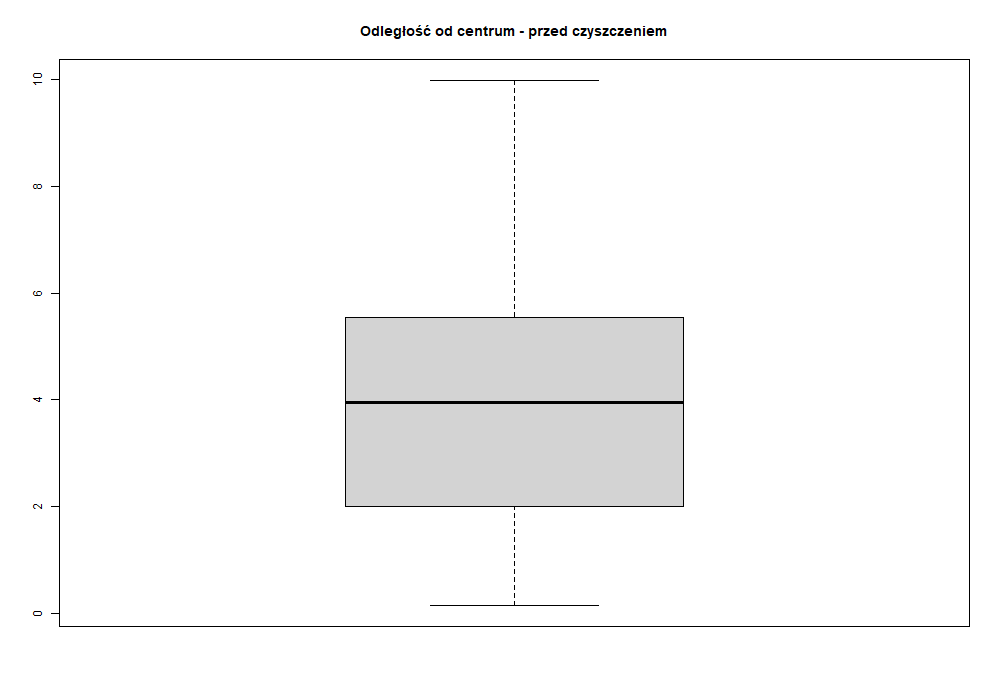
\includegraphics[width=\textwidth]{boxplot_centreDistance.png}
    \caption{Odległość od centrum przed czyszczeniem}
\end{minipage}
\hfill
\begin{minipage}{0.48\textwidth}
    \centering
    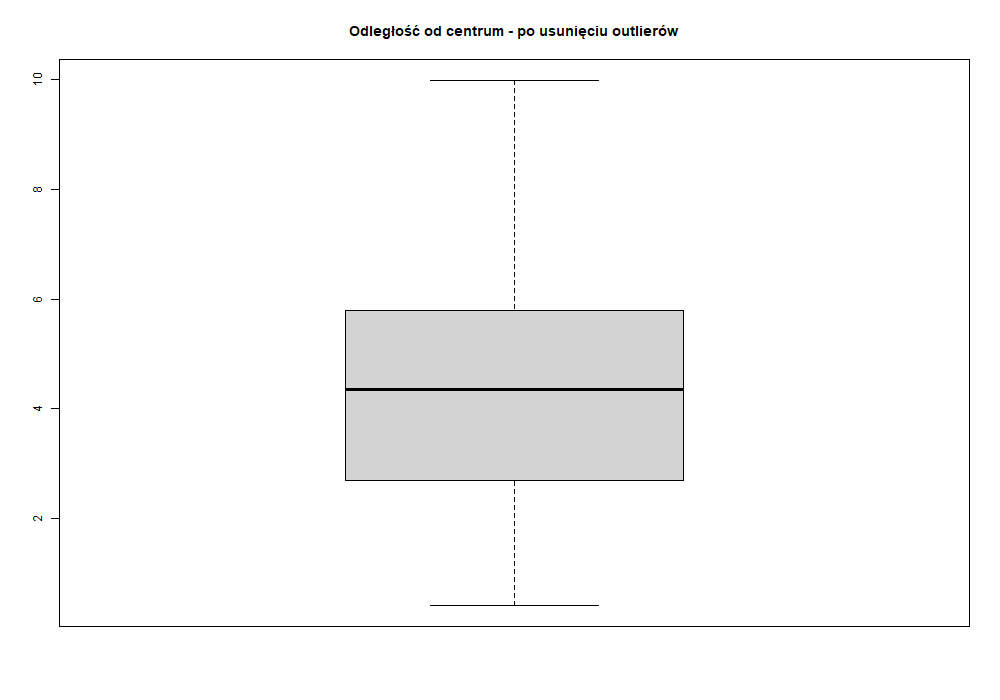
\includegraphics[width=\textwidth]{boxplot_centreDistance_clean.png}
    \caption{Odległość od centrum po czyszczeniu}
\end{minipage}

\end{figure}
\chapter{Opis metod}

W niniejszym rozdziale przedstawiono dwie metody analizy skupień zastosowane w ramach projektu, tj. algorytm k-średnich (K-means) oraz hierarchiczną analizę skupień metodą aglomeracyjną. Metody te należą do najczęściej stosowanych technik uczenia nienadzorowanego i umożliwiają grupowanie obiektów na podstawie ich podobieństwa mierzonego w przestrzeni wielowymiarowej.

\section{Algorytm K-means}

\subsection{Opis metody}

Algorytm K-means jest jedną z najczęściej stosowanych metod analizy skupień, której celem jest podział zbioru danych na \(k\) rozłącznych klastrów w taki sposób, aby minimalizować zróżnicowanie wewnątrz poszczególnych grup.

Dla zbioru obserwacji \(X = \{x_1, x_2, \dots, x_n\}\) algorytm minimalizuje funkcję:

\[
J = \sum_{i=1}^{k} \sum_{x_j \in C_i} \|x_j - \mu_i\|^2
\]

gdzie:
\begin{itemize}
    \item \(k\) -- liczba klastrów,
    \item \(C_i\) -- i-ty klaster,
    \item \(x_j\) -- obserwacja,
    \item \(\mu_i\) -- centroid klastra,
    \item \(\|\cdot\|\) -- odległość euklidesowa.
\end{itemize}

Algorytm działa iteracyjnie, naprzemiennie przypisując obserwacje do najbliższych centroidów oraz aktualizując ich położenie jako średnią arytmetyczną przypisanych punktów. Proces ten powtarzany jest do momentu osiągnięcia zbieżności.

\subsection{Interpretacja klastrów}

Wyniki algorytmu K-means polegają na przypisaniu każdej obserwacji do jednego z \(k\) klastrów. Każdy klaster reprezentowany jest przez centroid, który można interpretować jako „typową” obserwację w danej grupie.

W kontekście analizy rynku nieruchomości klastry można interpretować jako segmenty mieszkań o podobnych cechach, takich jak cena, powierzchnia, liczba pokoi czy lokalizacja.

Interpretacja klastrów pozwala na identyfikację różnych segmentów rynku, np. mieszkań:
\begin{itemize}
    \item o wysokim standardzie i dużej powierzchni,
    \item średniego segmentu cenowego,
    \item małych mieszkań o niższej cenie i gorszej lokalizacji.
\end{itemize}

Dzięki temu możliwe jest nie tylko grupowanie danych, ale również ich praktyczna interpretacja ekonomiczna, co stanowi główną wartość analizy skupień w niniejszym projekcie.

\subsection{Dobór liczby klastrów}

Jednym z kluczowych etapów algorytmu K-means jest wybór odpowiedniej liczby klastrów \(k\), ponieważ metoda ta nie wyznacza tej wartości automatycznie.

W niniejszej pracy zastosowano metodę tzw. \textit{elbow method} (metody łokcia), która polega na analizie wartości funkcji celu (sumy kwadratów odległości obserwacji od centroidów) dla różnych wartości \(k\).

Dla każdej liczby klastrów obliczono miarę:

\[
J(k) = \sum_{i=1}^{k} \sum_{x_j \in C_i} \|x_j - \mu_i\|^2
\]

Następnie analizowano, jak zmienia się wartość \(J(k)\) wraz ze wzrostem liczby klastrów.

Wraz ze wzrostem \(k\) wartość błędu maleje, jednak po pewnym momencie tempo tej poprawy znacząco spada. Punkt ten, określany jako \textit{łokieć}, uznaje się za optymalną liczbę klastrów, ponieważ dalsze zwiększanie liczby grup nie przynosi istotnej poprawy jakości podziału danych.

Zastosowanie tej metody pozwala na kompromis pomiędzy jakością grupowania a jego złożonością interpretacyjną.

\section{Analiza hierarchiczna klastrów}

\subsection{Opis metody}

Analiza hierarchiczna klastrów (ang. \textit{hierarchical clustering}) jest metodą grupowania danych, która nie wymaga wcześniejszego określenia liczby klastrów. Zamiast tego buduje ona hierarchię skupień w postaci drzewa zależności, tzw. dendrogramu.

Metoda ta rozpoczyna się od traktowania każdej obserwacji jako osobnego klastra, a następnie w kolejnych krokach łączy najbardziej podobne grupy, aż do uzyskania jednego wspólnego klastra obejmującego wszystkie obserwacje.

Do określenia podobieństwa pomiędzy obserwacjami wykorzystywana jest miara odległości, najczęściej odległość euklidesowa:

\[
d(x_i, x_j) = \sqrt{\sum_{p=1}^{m} (x_{ip} - x_{jp})^2}
\]

gdzie:
\begin{itemize}
    \item \(x_i, x_j\) -- obserwacje,
    \item \(m\) -- liczba zmiennych,
    \item \(d(x_i, x_j)\) -- odległość pomiędzy obserwacjami.
\end{itemize}

W procesie łączenia klastrów istotną rolę odgrywa metoda wiązania (ang. \textit{linkage}), która określa sposób obliczania odległości pomiędzy grupami. W niniejszej pracy zastosowano metodę wiązania Warda, która minimalizuje wzrost wariancji wewnątrz klastrów przy każdym połączeniu.

\subsection{Interpretacja metody}

Wynikiem analizy hierarchicznej jest dendrogram, czyli drzewo przedstawiające kolejność łączenia obserwacji i klastrów.

Przecięcie dendrogramu na wybranym poziomie pozwala uzyskać określoną liczbę klastrów, które można interpretować jako segmenty danych o podobnych cechach.

W kontekście analizy rynku nieruchomości metoda ta pozwala na identyfikację naturalnej struktury danych oraz ocenę, jak poszczególne grupy mieszkań łączą się ze sobą w zależności od ich podobieństwa.

Dodatkową zaletą analizy hierarchicznej jest możliwość wizualnej oceny relacji pomiędzy obserwacjami, co ułatwia interpretację struktury danych oraz wybór liczby klastrów.

\section{Podsumowanie metod}

Zastosowanie dwóch różnych metod analizy skupień pozwala na porównanie stabilności oraz jakości otrzymanych wyników. K-means zapewnia efektywność obliczeniową i prostotę implementacji, natomiast metoda hierarchiczna umożliwia bardziej szczegółową analizę struktury danych i wybór liczby klastrów na podstawie dendrogramu.

\section{Przegląd literatury dotyczącej metod}

Metoda K-means została po raz pierwszy formalnie opisana przez Stuarta Lloyda w 1957 roku w kontekście kompresji sygnałów, a następnie szeroko rozpowszechniona w literaturze statystycznej i uczeniu maszynowym.

Jedną z najczęściej cytowanych prac dotyczących algorytmu K-means jest publikacja MacQueena, który w 1967 roku wprowadził pojęcie klastrów w kontekście analizy danych:

\begin{itemize}
    \item MacQueen, J. (1967). \textit{Some Methods for classification and Analysis of Multivariate Observations}. Proceedings of the Fifth Berkeley Symposium on Mathematical Statistics and Probability.
\end{itemize}

Współczesne ujęcie metod analizy skupień, w tym zarówno metody K-means, jak i metod hierarchicznych, zostało szczegółowo opisane w literaturze podręcznikowej dotyczącej eksploracyjnej analizy danych, m.in.:

\begin{itemize}
    \item Jain, A. K., Murty, M. N., \& Flynn, P. J. (1999). \textit{Data Clustering: A Review}. ACM Computing Surveys.
    \item Hastie, T., Tibshirani, R., \& Friedman, J. (2009). \textit{The Elements of Statistical Learning}. Springer.
\end{itemize}

Prace te stanowią podstawę teoretyczną dla zastosowanych w niniejszym projekcie metod analizy skupień oraz ich interpretacji w kontekście danych wielowymiarowych.
\chapter{Wyniki}

(w postaci tabelarycznej i/lub graficznej oraz omówienie wyników)

\chapter{Podsumowanie}

(ocena realizacji celu, odniesienie do pozycji z przeglądu literatury)

\chapter{Bibliografia}



\end{document}
